\documentclass[a4paper]{article}

%\usepackage[english]{babel}
%\usepackage[utf8]{inputenc}
\usepackage{graphicx}
\usepackage{epsfig}
%\usepackage{amsmath}
\usepackage{graphicx}
\usepackage[colorinlistoftodos]{todonotes}
\usepackage{a4}
%\usepackage{amssymb}
\usepackage{color}
\usepackage{lineno}
\usepackage{ulem}
\usepackage{enumerate}
\usepackage{comment}

\usepackage[left=2.5cm,right=2cm,top=2.5cm,bottom=2.cm]{geometry} 

%% for long url reference
\usepackage{hyperref}
\usepackage{url}
\makeatletter
\def\url@mystyle{%
  \@ifundefined{selectfont}{\def\UrlFont{\sf}}{\def\UrlFont{\small\ttfamily}}}
\makeatother
\urlstyle{my}



\renewcommand{\thefootnote}{\alph{footnote}}
\renewcommand{\topfraction}{.99}
\renewcommand{\bottomfraction}{.99}

\title{Momentum based dE/dX Calibration of LArIAT for Run I and Run II}

%%%%%%%%%%%%%%%%%%%%%%%%%%%%%%%%%
\begin{document}
%%%%%%%%%%%%%%%%%%%%%%%%%%%%%%%%%
\def\Journal#1#2#3#4{{#1} {\bf #2}, #3 (#4)}
\def\etal{{\it et\ al.}}
\def\numunue{\nu_\mu\rightarrow\nu_e}
\def\numunutau{\nu_\mu\rightarrow\nu_\tau}
\def\nuebar{\bar\nu_e}
\def\nue{\nu_e}
\def\nutau{\nu_\tau}
\def\numubar{\bar\nu_\mu}
\def\numu{\nu_\mu}
\def\ra{\rightarrow}
\def\numubarnuebar{\bar\nu_\mu\rightarrow\bar\nu_e}
\def\nuebarnumubar{\bar\nu_e\rightarrow\bar\nu_\mu}
\def\osc{\rightsquigarrow}
\def\inteni{{\cal I}_{pot}}
\def\fmerit{{\cal F}}
%%%%%%%%%%%%%%%%%%%%%%%%%%%%%%%%%
\begin{flushright}
{\tt version 0.5}\\ 
\today
\end{flushright}
\vspace*{0.6cm}
%%%%%%%%%%%%%%%%%%%%%%%%%%%%%%%%%
%\linenumbers
%%%%%%%%%%%%%%%%%%%%%%%%%%%%%%%%%
\begin{center}
{\Large \bf Momentum based dE/dX Calibration of LArIAT for Run I and Run II} 
\vspace*{1.6cm}
\setcounter{footnote}{0}  
\def\A{\kern+.6ex\lower.42ex\hbox{$\scriptstyle \iota$}\kern-1.20ex a}
\def\E{\kern+.5ex\lower.42ex\hbox{$\scriptstyle \iota$}\kern-1.10ex e}
\small
\newcommand{\Aname}[2]{#1}
\def\titlefoot#1{\vspace{-0.3cm}\begin{center}{\bf #1}\end{center}}

\Aname{J.~Asaadi}{UTA},

\titlefoot{University of Texas at Arlington\label{UTA}}
%\vspace{-0.1cm}

\Aname{E. Gramellini}{Yale},

\titlefoot{Yale University\label{Yale}}
%\vspace{-0.1cm}

\Aname{G. Pullium}{Syracuse},

\titlefoot{Syracuse University\label{Syracuse}}
%\vspace{-0.1cm}

\end{center}
\vspace*{1cm}


%%%%%%%%%%%%%%%%%%%%%%%%%%%%%%%%%
%% ABSTRACT
%%%%%%%%%%%%%%%%%%%%%%%%%%%%%%%%%
%\newpage
\begin{abstract}

We present the calibration technique of parameterizing the energy deposited per unit length (dE/dX) as a function of momentum used to calibrate both the data and Monte Carlo samples for Run-I and Run-II. This calibration is done for a sample of $\pi, \mu$, and protons from the beamline and cross-checked using a sample of cosmic rays. The results for this calibration along with the derived calibration constants are presented.

\end{abstract} 

%%%%%%%%%%%%%%%%%%%%%%%%%%%%%%%%%
%% Table of content
%%%%%%%%%%%%%%%%%%%%%%%%%%%%%%%%%
\newpage
\tableofcontents


%%%%%%%%%%%%%%%%%%%%%%%%%%%%%%%%%
%% SECTION 1: Introduction
%%%%%%%%%%%%%%%%%%%%%%%%%%%%%%%%%
%%\section{Introduction and physics case} 
\newpage
\section{Introduction}\label{sec:Introduction}

Here we present the results of the calorimetry tuning done for a sample of data and Monte Carlo spanning Run I and Run II of the LArIAT experiment. This calibration method is predicated on the Bethe-Block description of the mean rate of energy loss for various particle species. This is best represented by Figure \ref{fig:PDGEnergyLoss}, taken from the Particle Data Group \cite{PDG}.

\begin{figure}[htb]
\centering
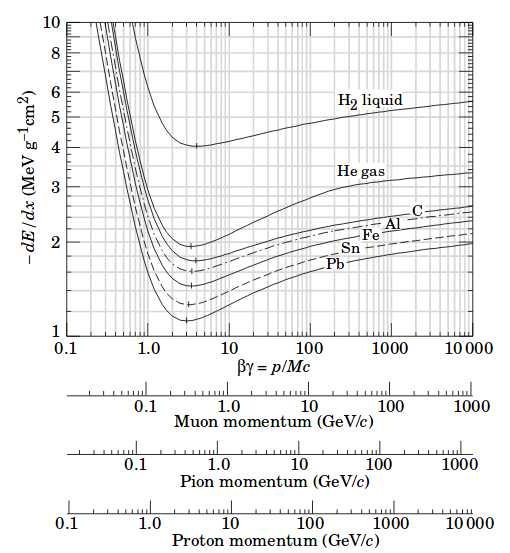
\includegraphics[width=0.50\textwidth]{images/PDGdEdX.png}
\caption{Mean energy loss in various materials over a range of particle momentums as produced in Reference \cite{PDG}.}
\label{fig:PDGEnergyLoss}
\end{figure}

Using the tables provided by the PDG for liquid argon (\cite{PDG-Argon}), we calculate the theoretical values for pions ($\pi$), muons ($\mu$), and protons ($p$) in the momentum range most relevant for LArIAT, shown in Figure \ref{fig:PDGEnergyLossArgon}.

\begin{figure}[htb]
\centering
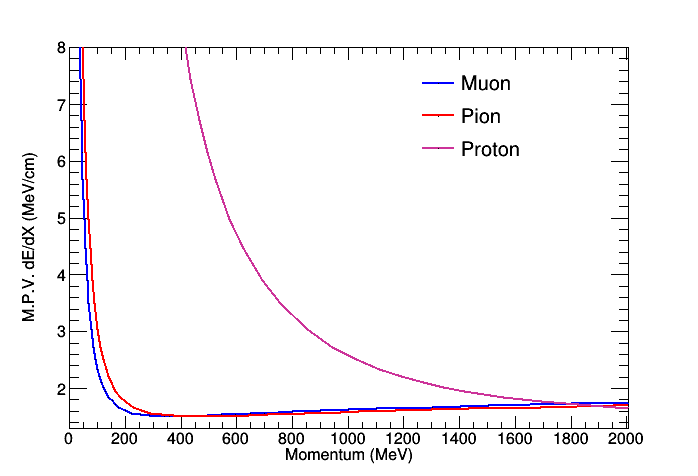
\includegraphics[width=0.50\textwidth]{images/dEdXvsMomentumTemplate}
\caption{Mean energy loss for pions, muons, and protons in liquid argon over the momentum range most relvant for LArIAT.}
\label{fig:PDGEnergyLossArgon}
\end{figure}

Using the predictions in Figure \ref{fig:PDGEnergyLossArgon}, allows us to tune the calorimetry constants used to convert the ADC to charge. The goal is to have the data and MC agree across the broad range of momentum. This tuning is done in addition to the wire-by-wire corrections (described in detail in \href{http://lartpc-docdb.fnal.gov:8080/cgi-bin/RetrieveFile?docid=1994&filename=investigation-uniformity-observed_v3.pdf&version=2}{doc-DB 1994}) and the usual lifetime corrections (described in detail in \href{http://lartpc-docdb.fnal.gov:8080/cgi-bin/ShowDocument?docid=1804}{docDB-1804}) which are used here and a more detailed treatment is left to their corresponding technical notes.

%%%%%%%%%%%%%%%%%%%%%%%%%%%%%%%%%%%%%%%%%%%%%%%%%%%%%%%%%%%
\subsection{Calibration Method Overview}\label{sec:MethodOverview}
%%%%%%%%%%%%%%%%%%%%%%%%%%%%%%%%%%%%%%%%%%%%%%%%%%%%%%%%%%%

In this section, we will describe the methodology we use to select our samples and tune the calorimetry constants. Details specific to any one sample will be described in Section  \ref{sec:EventSelection} and instead we will present the general method and how it is applied. 

The basic idea of this calibration technique is to utilize portion of a track within the LArTPC that has a well known momentum and particle species to measure the energy deposited per unit length (dE/dX) as recorded inside the TPC. Once a sample of particles dE/dX has been measured at various momentums, we then tune to calorimetry constants within the reconstruction software align these measured values to match the theoretical ones found in Figure \ref{fig:PDGEnergyLossArgon}.

Since various electronics changes and fixes to the PMT system were done between Run-I and Run-II, we derive calibration constants independently for both of these run periods. These calibration constants are the factors which convert the charge collected (dQ) to energy (dE). The details of how the calorimetry package works is beyond the scope of this note and is given in \href{http://lartpc-docdb.fnal.gov:8080/cgi-bin/ShowDocument?docid=2444}{docDB-2444}.

The calibration procedure follows the following basic steps:
\begin{itemize}

\item \textbf{Particle Identification in the beamline:}

We first select a sample of beamline events that correspond to either a sample of $\pi, \mu, e$ or protons. This is done by selecting based on the measured time-of-flight (TOF) vs momentum as measured in the wire chambers. We start by requiring the tracks reconstructed in the wire chamber satisfy the criteria known as a ``picky'' track, meaning the track reconstructed from the four wire chambers has a hit in each wire chamber. In these events, one and only one wire chamber track can be reconstructed per event. These tracks have a more accurate measure of the particle momentum than the ``high yield'' tracks which only require hits in three out of four of the wire chamber tracks and can have mulitple wire chamber tracks reconstructed per event. The ``high yield'' sample is used as a cross-check with more statistics once the calibration constants are found.

The wire chamber track is extrapolated to the front face of the LArTPC giving a $x, y$ position expected for the track in the TPC. A simple flat correction to the energy loss by the particle as it traverses the material between the last wire chamber and the front face of the LArTPC.

For the Monte Carlo, no such beamline identification is done and instead we use the data-driven Monte Carlo (DDMC), which constructs the momentum and angular distributions for the single particle MC, and launches particles from the position of the fourth wire chamber (WC4) towards the TPC. We utilize the Monte Carlo truth for the position and momentum of the Monte Carlo particles as they enter the TPC.

\item \textbf{Matching LArTPC tracks to the wire chamber tracks:}

For each track reconstructed inside the TPC, the most upstream trajectory point (smallest $z$ position) is found. For that point we have it's $x, y, z$ as well as the calculated $p_{x}, p_{y}, and p_{z}$ (which is used to calculate the tracks $\theta, \phi$. Using this as well as the wire chamber tracks extrapolated $x, y, \theta, \phi$ we then select the event if there is one and only one TPC track which matches the wire chamber track. The exact matching criteria is given in Section \ref{sec:EventSelection}.

We now have the initial momentum (corrected for energy loss due to the upstream material) of the TPC track which we can use for our calibration.

For the Monte Carlo, the ``wire chamber'' matching is done treating the true position of the MC particle as it enters the TPC as the ``wire chamber'' track. The rest of the matching proceeds just as before.

\item \textbf{dE/dX sampling:}



\end{itemize}

%%%%%%%%%%%%%%%%%%%%%%%%%%%%%%%%%
%% SECTION 2: Data Samples
%%%%%%%%%%%%%%%%%%%%%%%%%%%%%%%%%
\section{Data Samples}

Data Samples \cite{Willis:1974gi}. 


%%%%%%%%%%%%%%%%%%%%%%%%%%%%%%%%%
%% SECTION 3
%%%%%%%%%%%%%%%%%%%%%%%%%%%%%%%%%
%%\section{The Concept of ArgonCube TPC module}
%\section{Results}\label{sec:Results}


%%%%%%%%%%%%%%%%%%%%%%%%%%%%%%%%%%%%%%%%%%%%%%%%%%%%%%%
\subsection{Run-I Data}\label{sec:RunI}
%%%%%%%%%%%%%%%%%%%%%%%%%%%%%%%%%%%%%%%%%%%%%%%%%%%%%%%
Table \ref{tab:RunICutSummary} summarizes the number of events which are selected to use as the calibration or validation samples in order to tune our calorimetry constants.

%%% Put event reduction tables here 
\begin{table}[htb]
	\begin{center}
	\resizebox{0.98\textwidth}{!}{%
	\begin{tabular}{|c|c|c|c|c|c|}
	\hline
	%\multicolumn{5}{|c|}{\textbf{Summary of inclusive NC $\pi^{0}$ Event Selection Cuts}} \\
	%\hline \hline
	  \textbf{Event Selection} & Run-I Negative Polarity & Run-I Negative Polarity &  Run-I Positive Polarity & Run-I Positive Polarity & Run-I Positive Polarity  \\
	   & $\pi^{-}, \mu^{-}, e^{-}$ & $K^{-}$ & $\pi^{+}, \mu^{+}, e^{+}$ & $K^{+}$ & Proton  \\
	\hline
	Beam Filter & 113,042 & 113,042 & 140,954 & 140,954 & 140,954 \\
	\hline
	Mass Selection & 5,909 & 63 & 5,349 & 346 &  9,104 \\
	\hline
	$>$ 1 Track Reconstructed in the TPC & 5,722  & 58 & 5,223 & 337  & 8,062  \\
	\hline
	$<$ 3 Tracks Reconstructed &  &  &  &  &  \\
	with length $<$ 5~cm & 4,323 & 45 & 4,058 &  263 & 6,561  \\
	\hline
	Unique match between WC and TPC Track & 2,464 & 17 & 2,446  & 120 & 3,373  \\
	\hline
	\hline
	\end{tabular}}
	\caption{Summary of event selection applied to the calibration sample for Run-I data.} \label{tab:RunICutSummary}
	\end{center}
\end{table}

Figure \ref{fig:Run1NegPosPickyTrkTotal} shows the total calibration for Run-I data samples using the calorimetry constants \verb!physics.producers.calo.CaloAlg.CalAreaConstants: [0.025,0.052]!. The results only show the tuning of the collection plane values. Due to the limited statistics in the kaon sample, bins in momentum with too few entries were omitted from the plot due to the poor fit values returned. 

In the sub-sections below we focus in on the various sub-samples to show the results of the tuning in detail.

\begin{figure}[h!]
\centering
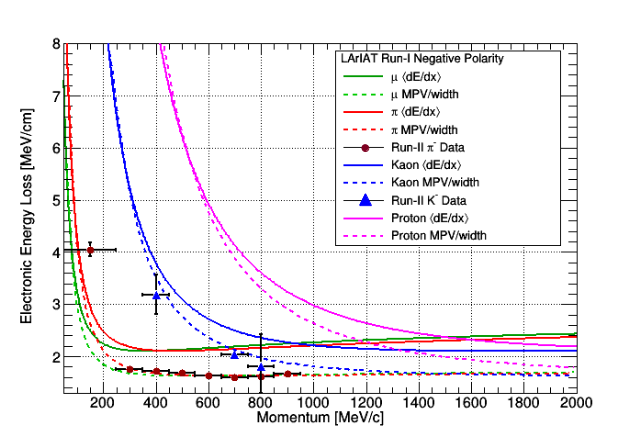
\includegraphics[width=0.75\textwidth]{images/RunINegTotaldEdXvsMomentum.png}
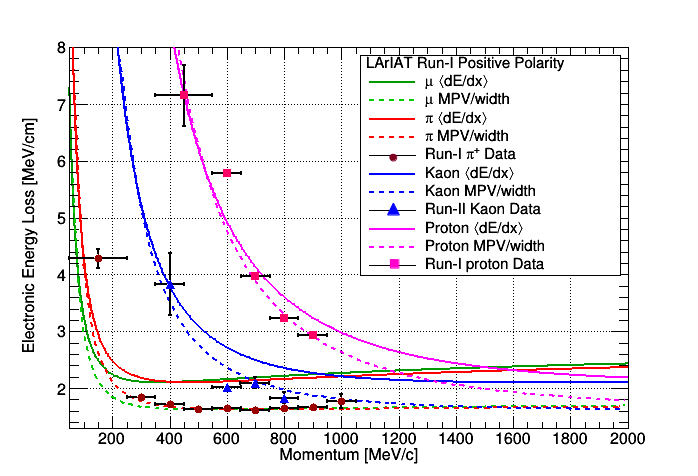
\includegraphics[width=0.75\textwidth]{images/RunIPosTotaldEdXvsMomentum.png}
\caption{(Left) dE/dX vs Momentum for Run-I Negative Polarity Picky Tracks: $\pi^{-}, \mu^{-}, e^{-}$ and $K^{-}$ sample ,(Right) dE/dX vs Momentum for Run-I Positive Polarity Picky Tracks: $\pi^{+}, \mu^{+}, e^{+}$ and $K^{+}$, and Proton sample. }
\label{fig:Run1NegPosPickyTrkTotal}
\end{figure}

\clearpage

%%%%%%%%%%%%%%%%%%%%%%%%%%%%%%%%%%%%%%%%%%%%%%%%%%%%%%%
\subsubsection{Negative Polarity Picky Tracks: $\pi^{-}, \mu^{-}, e^{-}$}\label{sec:Run1NegPickyTrkPiMuE}
%%%%%%%%%%%%%%%%%%%%%%%%%%%%%%%%%%%%%%%%%%%%%%%%%%%%%%%

The sample of 2,464 negative polarity $\pi^{-}, \mu^{-}, e^{-}$ picky tracks was used to tune the calorimetry constants for Run-I. After several iterations the calo constants \verb!physics.producers.calo.CaloAlg.CalAreaConstants: [0.025,0.052]! were chosen. Figure \ref{fig:Run1NegPickyTrkPiMuEResults} shows the dE/dX vs momentum and the aggregate dE/dX distribution obtained with these calorimetry constants.

\begin{figure}[htb]
\centering
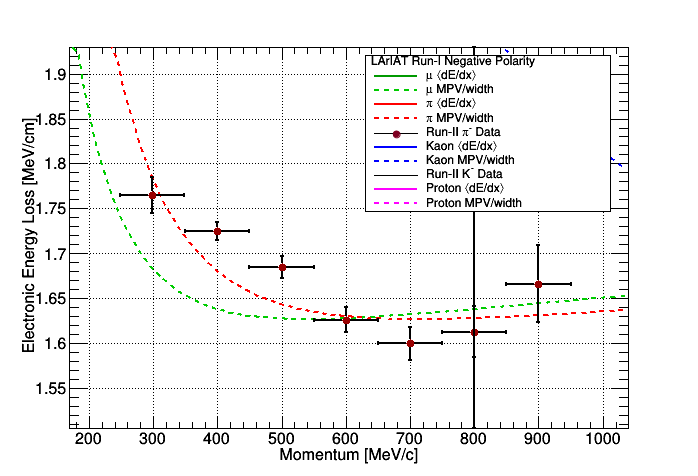
\includegraphics[width=0.48\textwidth]{images/dEdXvsMomentumNegPolRun1FineBin2.png}
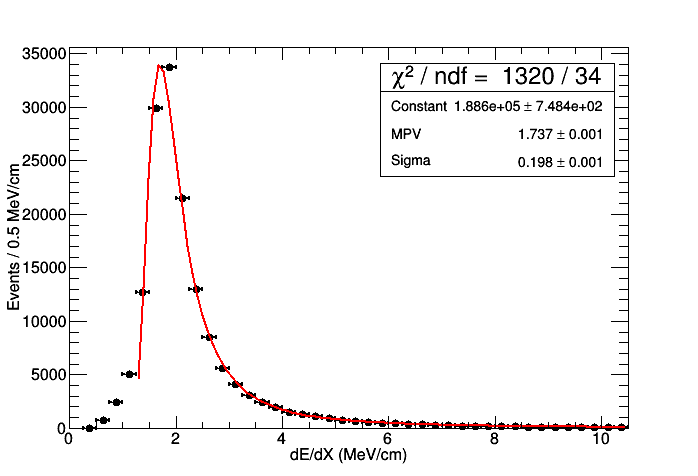
\includegraphics[width=0.48\textwidth]{images/dEdXRun1NegPolFinal.png}
\caption{(Top) dE/dX vs Momentum for Negative Polarity Picky Tracks: $\pi^{-}, \mu^{-}, e^{-}$ sample ,(Bottom) dE/dX for the entire sample of uniquely matched tracks in the Negative Polarity Picky Tracks: $\pi^{-}, \mu^{-}, e^{-}$ sample }
\label{fig:Run1NegPickyTrkPiMuEResults}
\end{figure}

The distributions here generally agree with the theoretical curve for a sample of pions and muons (as there is expected to be a small contamination of the pion beam with through going muons. The MPV for the entire sample of 1.737 MeV/cm is slightly higher than the expected value of 1.65 MeV/cm for a mean momentum of $\sim$500 MeV as was present for this sample, shown in Figure \ref{fig:Run1NegPickyTrkPiMuEMomentumSpec}.

\begin{figure}[htb]
\centering
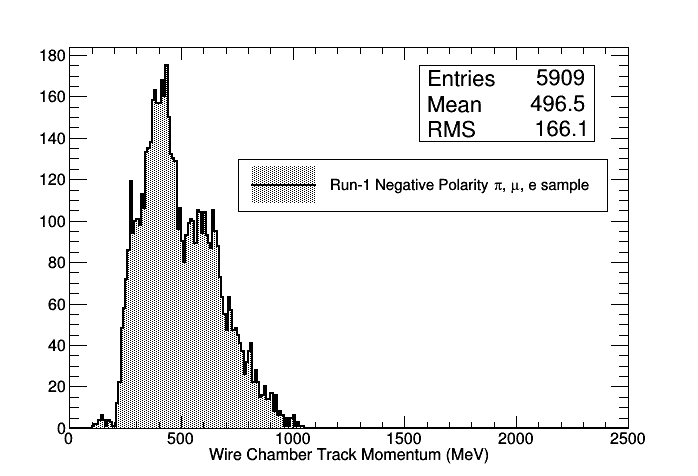
\includegraphics[width=0.55\textwidth]{images/WCTrkMomentumRun1NegPiMuE.png}
\caption{Wire chamber track momentum spectrum for the Run-I Negative Polarity Picky Tracks: $\pi, \mu, e$ sample  }
\label{fig:Run1NegPickyTrkPiMuEMomentumSpec}
\end{figure}

Even with this slight inconsistency between the expected MPV for the mean momentum of the sample and the measured value, these calorimetry constants do provide a good characterization of the overall Bethe-Bloch curve and, as we will see in the other samples, work well for kaons, protons, and positive pions.

%%%%%%%%%%%%%%%%%%%%%%%%%%%%%%%%%%%%%%%%%%%%%%%%%%%%%%%
\subsubsection{Negative Polarity Picky Tracks: $K^{-}$}\label{sec:Run1NegPickyTrkKaonMinus}
%%%%%%%%%%%%%%%%%%%%%%%%%%%%%%%%%%%%%%%%%%%%%%%%%%%%%%%
The sample of 17 negative polarity $K^{-}$ picky track events was used to first check the calibration constants provided in Section \ref{sec:Run1NegPickyTrkPiMuE}. This samples very small statistics limits the overall usefulness of this cross-check, but is provided here for completeness.

Figure \ref{fig:Run1NegPickyTrkKaonResults} shows the dE/dX vs momentum and the aggregate dE/dX distribution obtained with these calorimetry constants.

\begin{figure}[htb]
\centering
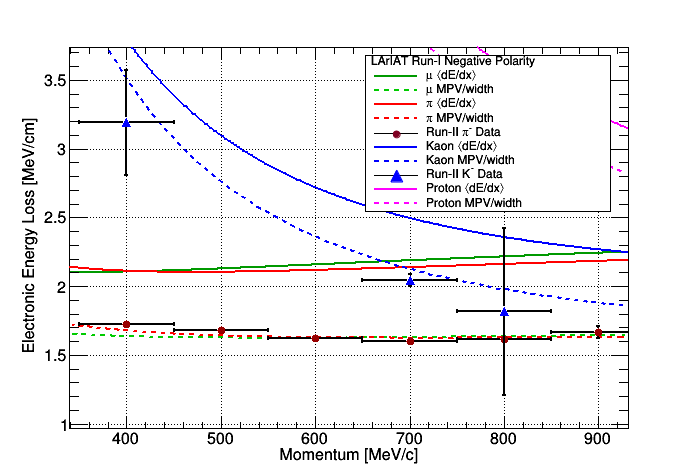
\includegraphics[width=0.48\textwidth]{images/dEdXvsMomentumNegPolRun1Kaon.png}
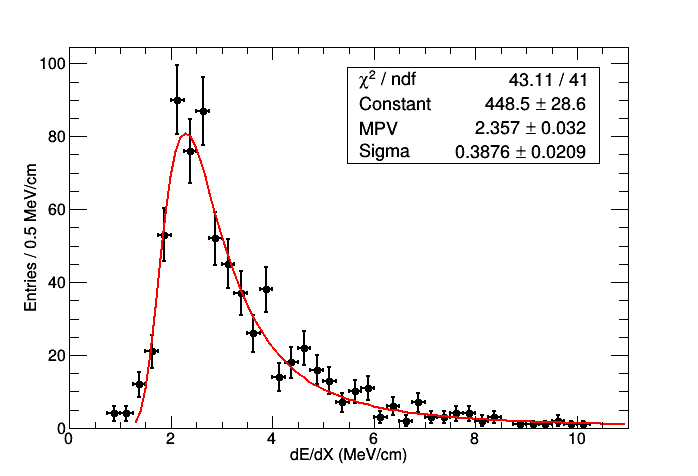
\includegraphics[width=0.48\textwidth]{images/dEdXKaonRunINegPol.png}
\caption{(Left) dE/dX vs Momentum for Negative Polarity Picky Tracks: $K^{-}$ sample ,(Right) dE/dX for the entire sample of uniquely matched tracks in the Negative Polarity Picky Tracks: $K^{-}$ sample }
\label{fig:Run1NegPickyTrkKaonResults}
\end{figure}

%%%%%%%%%%%%%%%%%%%%%%%%%%%%%%%%%%%%%%%%%%%%%%%%%%%%%%%
\subsubsection{Positive Polarity Picky Tracks: $\pi^{+}, \mu^{+}, e^{+}$}\label{sec:Run1PosPickyTrkPiMuE}
%%%%%%%%%%%%%%%%%%%%%%%%%%%%%%%%%%%%%%%%%%%%%%%%%%%%%%%

Using the same calibration constants derived in Section \ref{sec:Run1NegPickyTrkPiMuE}, we now look at the positive polarity sample of data collected in Run-I to validate the constants derived.  Figure \ref{fig:Run1PosPickyTrkPiMuEResults} shows the outcome for the sample of 2,446 positive polarity  $\pi^{+}, \mu^{+}, e^{+}$ events in Run-I.

\begin{figure}[htb]
\centering
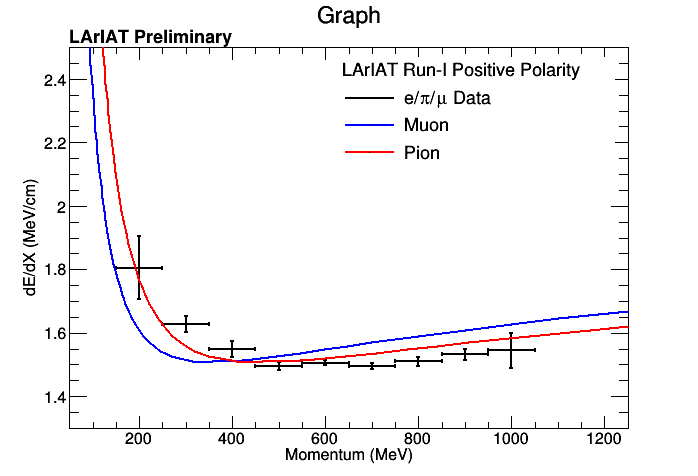
\includegraphics[width=0.48\textwidth]{images/dEdXvsMomentumPosPolRun1FineBin.png}
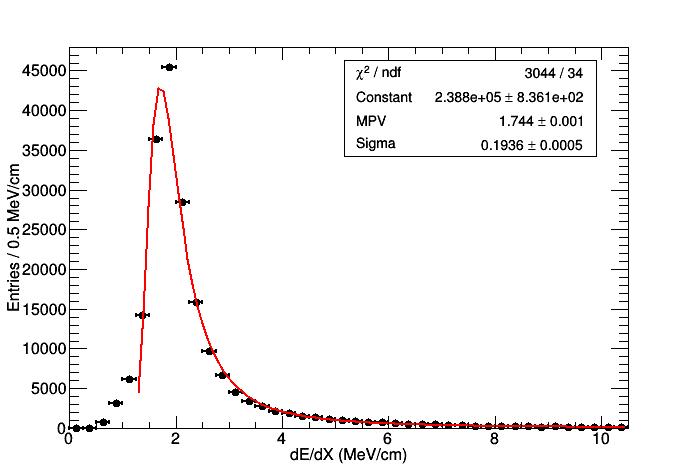
\includegraphics[width=0.48\textwidth]{images/dEdXPosPolRun1.png}
\caption{(Left) dE/dX vs Momentum for Positive Polarity Picky Tracks: $\pi^{+}, \mu^{+}, e^{+}$ sample ,(Right) dE/dX for the entire sample of uniquely matched tracks in the Positive Polarity Picky Tracks: $\pi^{+}, \mu^{+}, e^{+}$ sample }
\label{fig:Run1PosPickyTrkPiMuEResults}
\end{figure}

The distributions here also agree with the theoretical curve for a sample of pions and muons (as there is expected to be a small contamination of the pion beam with through going muons). The MPV for the entire sample of 1.74 MeV/cm which again is slightly higher than the expected 1.65 MeV/cm for a mean momentum of $\sim$650 MeV as was present for this sample, shown in Figure \ref{fig:Run1PosPickyTrkPiMuEMomentumSpec}. Despite this, teh data follows the Bethe-Bloch curve relatively well and validates the calibration constants derived with an independent sample of pions.

\begin{figure}[htb]
\centering
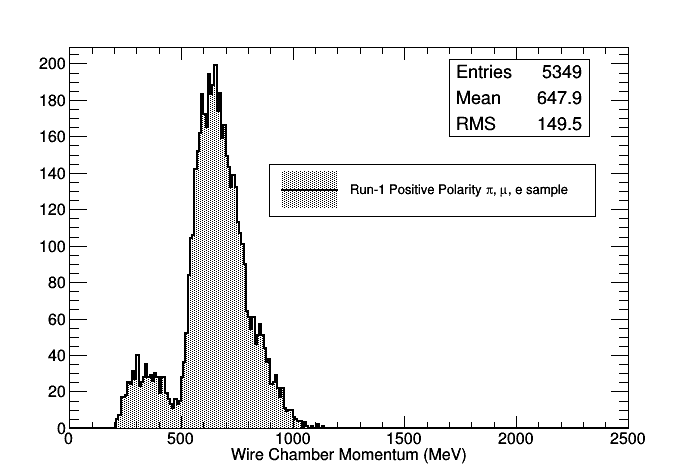
\includegraphics[width=0.55\textwidth]{images/WCTrkMomentumRun1PosPiMuE.png}
\caption{Wire chamber track momentum spectrum for the Run-I Positive Polarity Picky Tracks: $\pi, \mu, e$ sample}
\label{fig:Run1PosPickyTrkPiMuEMomentumSpec}
\end{figure}

%%%%%%%%%%%%%%%%%%%%%%%%%%%%%%%%%%%%%%%%%%%%%%%%%%%%%%%
\subsubsection{Positive Polarity Picky Tracks: $K^{+}$}\label{sec:Run1PosPickyTrkKaons}
%%%%%%%%%%%%%%%%%%%%%%%%%%%%%%%%%%%%%%%%%%%%%%%%%%%%%%%
The sample of 120 positive polarity $K^{+}$ picky track events was used to check the calibration constants provided in Section \ref{sec:Run1NegPickyTrkPiMuE}. This samples small statistics limits the overall usefulness of this cross-check, but is provided here for completeness.

Figure \ref{fig:Run1PosPickyTrkKaonResults} shows the dE/dX vs momentum and the aggregate dE/dX distribution obtained with these calorimetry constants.

\begin{figure}[htb]
\centering
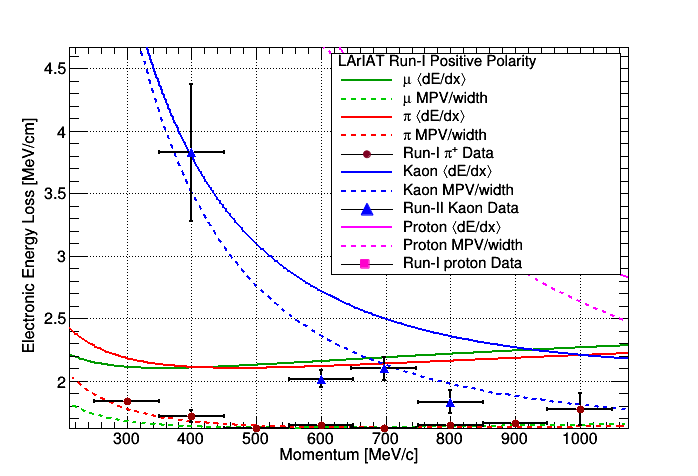
\includegraphics[width=0.48\textwidth]{images/dEdXvsMomentumPosPolRun1Kaon.png}
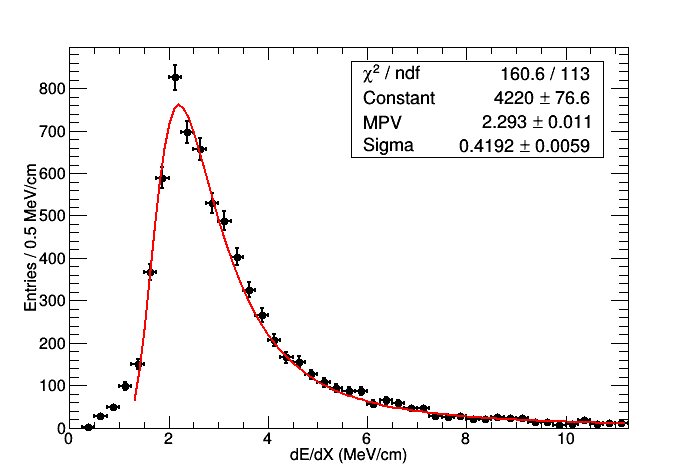
\includegraphics[width=0.48\textwidth]{images/dEdXKaonRunIPosPol.png}
\caption{(Left) dE/dX vs Momentum for Negative Polarity Picky Tracks: $K^{+}$ sample ,(Right) dE/dX for the entire sample of uniquely matched tracks in the Negative Polarity Picky Tracks: $K^{+}$ sample }
\label{fig:Run1PosPickyTrkKaonResults}
\end{figure}


%%%%%%%%%%%%%%%%%%%%%%%%%%%%%%%%%%%%%%%%%%%%%%%%%%%%%%%
\subsubsection{Positive Polarity Picky Tracks: Proton}\label{sec:Run1PosPickyTrkProton}
%%%%%%%%%%%%%%%%%%%%%%%%%%%%%%%%%%%%%%%%%%%%%%%%%%%%%%%

As a final cross-check for Run-1, a sample of protons is selected from the positive polarity picky track sample using the mass cut described in Section \ref{sec:EventSelection} using the same calibration constants derived in Section \ref{sec:Run1NegPickyTrkPiMuE}. The outcome of the calibration sample is shown in Figure \ref{fig:Run1PosPickyTrkProtonResults}.

\begin{figure}[htb]
\centering
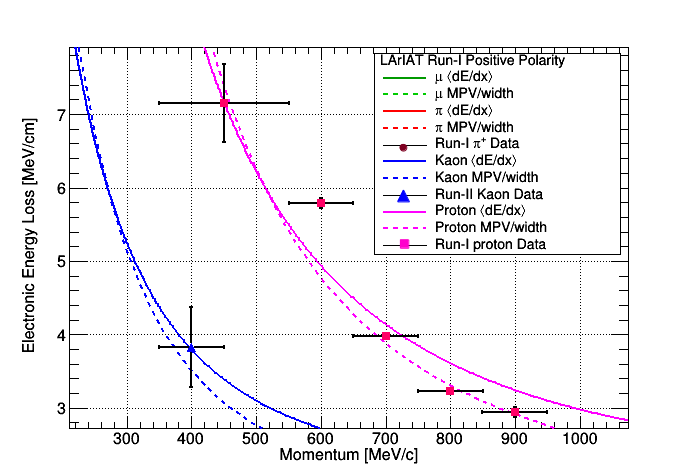
\includegraphics[width=0.48\textwidth]{images/dEdXvsMomentumPosPolRun1ProtonFineBin.png}
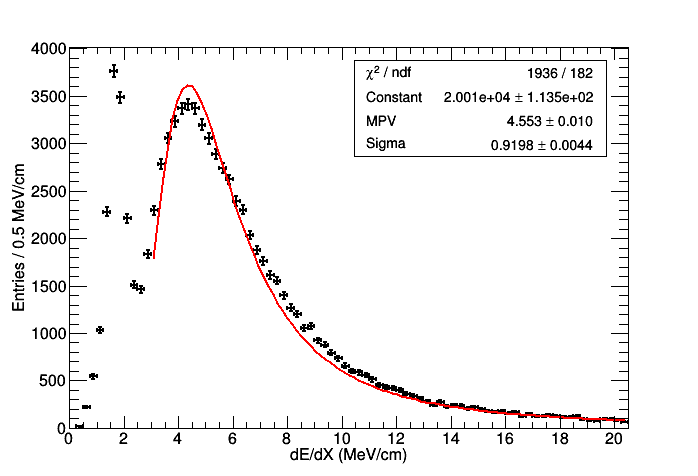
\includegraphics[width=0.48\textwidth]{images/dEdXPosPolRun1Proton.png}
\caption{(Left) dE/dX vs Momentum for Positive Polarity Picky Tracks proton sample ,(Right) dE/dX for the entire sample of uniquely matched tracks in the Positive Polarity Picky Tracks proton sample.}
\label{fig:Run1PosPickyTrkProtonResults}
\end{figure}

This sample differs slightly from the $\pi^{+}, \mu^{+}, e^{+}$ samples in that the ranges for the fits have been modified to exclude a contamination coming from minimum ionizing particles. This contamination can be seen in the RHS of Figure \ref{fig:Run1PosPickyTrkProtonResults} with the peak below 2~MeV/cm. Secondly, events with very low statistics in the momentum bins below 350~MeV are excluded from the LHS of Figure \ref{fig:Run1PosPickyTrkProtonResults} and the lowest bin is merged between 350 MeV and 550 MeV.

The MPV for the entire sample of 4.55 MeV/cm is slightly above expected value of 3.9 MeV/cm for a mean momentum of $\sim$730 MeV as was present for this sample, shown in Figure \ref{fig:Run1PosPickyTrkProtonMomentumSpec}. This slightly higher MPV is consistent with the results seen in the $\pi, \mu, e$ samples, but overall the data follows the Bethe-Bloch curve relatively well.

\begin{figure}[htb]
\centering
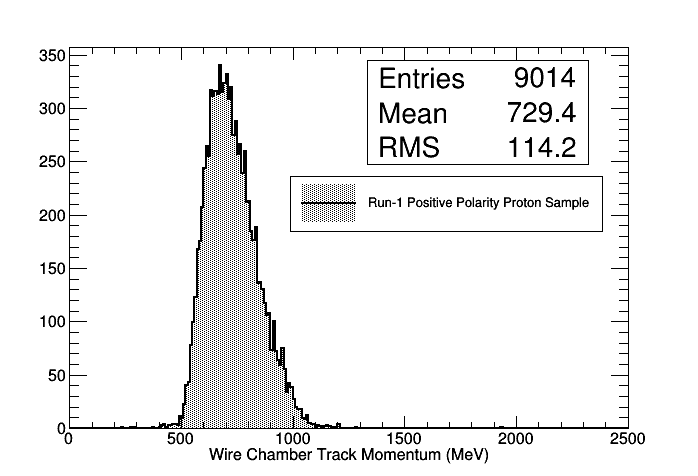
\includegraphics[width=0.55\textwidth]{images/WCTrkMomentumRun1PosProton.png}
\caption{Wire chamber track momentum spectrum for the Run-I Positive Polarity Picky Tracks proton sample  }
\label{fig:Run1PosPickyTrkProtonMomentumSpec}
\end{figure}

The overall agreement for these five samples using the calorimetry constants derived for Run-I validate the procedure and we now shift our attention to the applying the same methodology to Run-II data.

\newpage
%%%%%%%%%%%%%%%%%%%%%%%%%%%%%%%%%%%%%%%%%%%%%%%%%%%%%%%
\subsection{Run-II Data}\label{sec:RunII}
%%%%%%%%%%%%%%%%%%%%%%%%%%%%%%%%%%%%%%%%%%%%%%%%%%%%%%%
Table \ref{tab:RunIICutSummary} summarizes the number of events which are selected to use as the calibration or validation samples in order to tune our calorimetry constants for Run-II.

%%% Put event reduction tables here 
\begin{table}[htb]
	\begin{center}
	\resizebox{0.95\textwidth}{!}{%
	\begin{tabular}{|c|c|c|c|c|c|}
	\hline
	%\multicolumn{5}{|c|}{\textbf{Summary of inclusive NC $\pi^{0}$ Event Selection Cuts}} \\
	%\hline \hline
	  \textbf{Event Selection} & Run-II Negative Polarity & Run-II Negative Polarity  & Run-II Positive Polarity & Run-II Positive Polarity & Run-II Positive Polarity  \\
	   & $\pi^{-}, \mu^{-}, e^{-}$ & $K^{-}$ & $\pi^{+}, \mu^{+}, e^{+}$ & $K^{+}$ & Proton  \\
	\hline
	Beam Filter & 1,585,598 & 1,585,598  & 1,555,402 & 1,555,402  & 1,555,402 \\
	\hline
	Mass Selection & 124,965 & 835 & 89,561 & 4,289 & 94,210 \\
	\hline
	$>$ 1 Track Reconstructed in the TPC & 117,869 & 601 & 86,918 & 4,083 & 82,099  \\
	\hline
	$<$ 3 Tracks Reconstructed &  &  &  &  &  \\
	with length $<$ 5~cm & 88,717 & 428 & 69,509 & 3,385 & 68,847  \\
	\hline
	Unique match between WC and TPC Track & 48,076  & 216 & 43,547 & 1,719 & 36,278  \\
	\hline
	\hline
	\end{tabular}}
	\caption{Summary of event selection applied to the calibration sample.} \label{tab:RunIICutSummary}
	\end{center}
\end{table}

Figure \ref{fig:Run2NegPosPickyTrkTotal} shows the total calibration for Run-II data samples using the calorimetry constants \verb!physics.producers.calo.CaloAlg.CalAreaConstants: [0.022,0.0445]!. The results only show the tuning of the collection plane values. Due to the limited statistics in the kaon sample, bins in momentum with too few entries were omitted from the plot due to the poor fit values returned. 

\begin{figure}[h!]
\centering
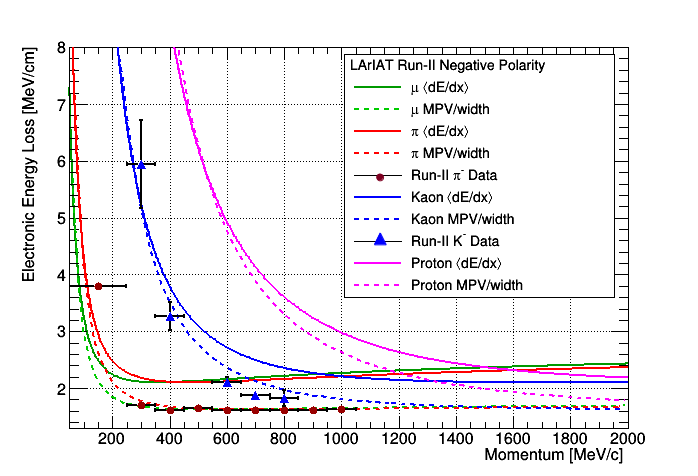
\includegraphics[width=0.75\textwidth]{images/RunIINegTotaldEdXvsMomentum.png}
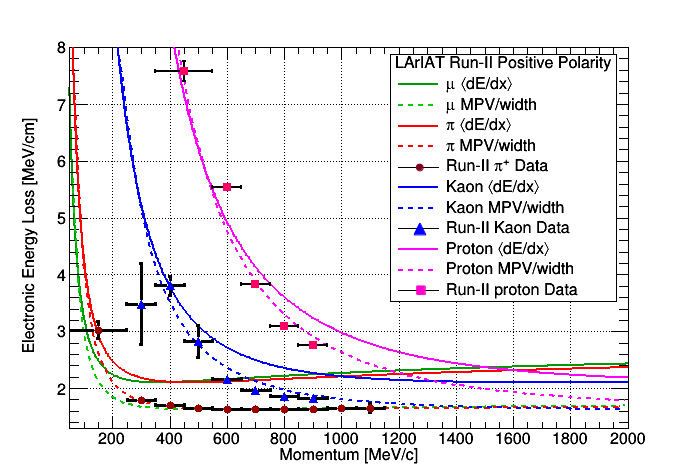
\includegraphics[width=0.75\textwidth]{images/RunIIPosTotaldEdXvsMomentum.png}
\caption{(Top) dE/dX vs Momentum for Run-II Negative Polarity Picky Tracks: $\pi^{-}, \mu^{-}, e^{-}$ and $K^{-}$ sample ,(Bottom) dE/dX vs Momentum for Run-II Positive Polarity Picky Tracks: $\pi^{+}, \mu^{+}, e^{+}$ and $K^{+}$, and Proton sample. }
\label{fig:Run2NegPosPickyTrkTotal}
\end{figure}

For Run-II data, a slightly different order was followed in tuning the calibration constants. For this set of data we began with positive polarity picky tracks  $\pi^{+}, \mu^{+}, e^{+}$ sample and then checked this tuning with $K^{+}$ and the proton sample before cross-checking with the negative polarity picky tracks  $\pi^{-}, \mu^{-}, e^{-}$ and $K^{-}$ sample. This was done to help ensure the samples weren't being biased in the tuning for the negative polarity pion inclusive cross-section sample.  The order is the method was applied is represented by the section numbering.

%%%%%%%%%%%%%%%%%%%%%%%%%%%%%%%%%%%%%%%%%%%%%%%%%%%%%%%
\subsubsection{Positive Polarity Picky Tracks: $\pi^{+}, \mu^{+}, e^{+}$}\label{sec:Run2PosPickyTrkPiMuE}
%%%%%%%%%%%%%%%%%%%%%%%%%%%%%%%%%%%%%%%%%%%%%%%%%%%%%%%

This sample of events was used to tune the calorimetry constants for Run-II. After several iterations the calo constants \verb!physics.producers.calo.CaloAlg.CalAreaConstants: [0.022,0.0445]! were chosen. Figure \ref{fig:Run2PosPickyTrkPiMuEResults} shows the dE/dX vs momentum and the aggregate dE/dX distribution obtained with these calorimetry constants.

\begin{figure}[htb]
\centering
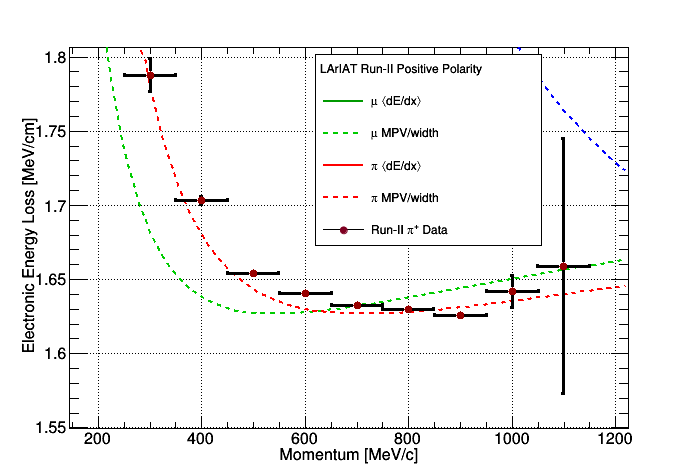
\includegraphics[width=0.48\textwidth]{images/dEdXvsMomentumPosPolRun2FineBin.png}
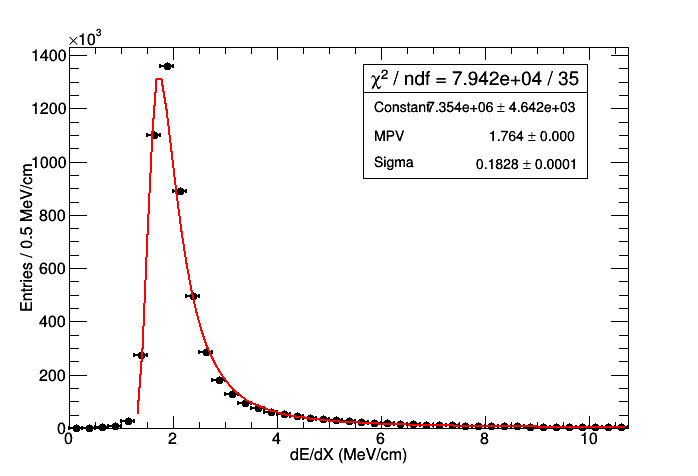
\includegraphics[width=0.48\textwidth]{images/dEdXPosPolRun2.png}
\caption{(Left) dE/dX vs Momentum for Positive Polarity Picky $\pi^{+}, \mu^{+}, e^{+}$ sample ,(Right) dE/dX for the entire sample of uniquely matched tracks in the Positive Polarity Picky $\pi^{+}, \mu^{+}, e^{+}$ sample }
\label{fig:Run2PosPickyTrkPiMuEResults}
\end{figure}

The distributions here generally agree with the theoretical curve for a sample of pions and muons (as there is expected to be a small contamination of the pion beam with through going muons. The MPV for the entire sample of 1.76 MeV/cm is slightly higher than the expected 1.63 MeV/cm for a mean momentum of $\sim$640 MeV as was present for this sample, shown in Figure \ref{fig:Run2PosPickyTrkPiMuEMomentumSpec}. While this agreement isn't great, the sample does clearly follow the expected Bethe-Bloch curve for the various momentum steps.

\begin{figure}[htb]
\centering
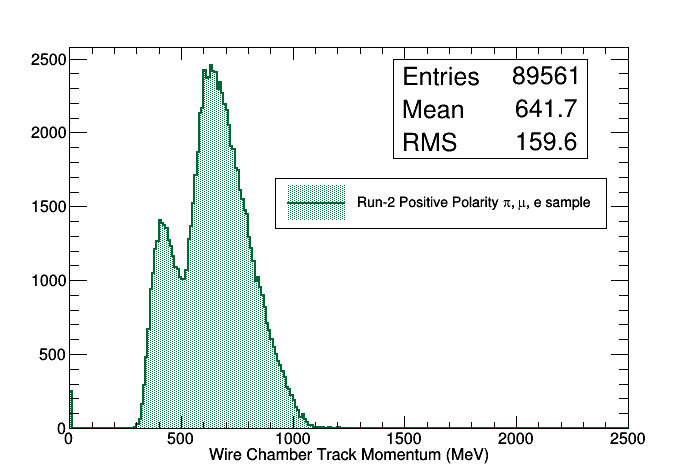
\includegraphics[width=0.55\textwidth]{images/WCTrkMomentumRun2PosPiMuE.png}
\caption{Wire chamber track momentum spectrum for the Run-II Positive Polarity Picky $\pi, \mu, e$ sample  }
\label{fig:Run2PosPickyTrkPiMuEMomentumSpec}
\end{figure}

%%%%%%%%%%%%%%%%%%%%%%%%%%%%%%%%%%%%%%%%%%%%%%%%%%%%%%%
\subsubsection{Positive Polarity Picky Tracks: $K^{+}$}\label{sec:Run2PosPickyTrkKaons}
%%%%%%%%%%%%%%%%%%%%%%%%%%%%%%%%%%%%%%%%%%%%%%%%%%%%%%%
The sample of 1,719 positive polarity $K^{+}$ picky track events was used to check the calibration constants provided in Section \ref{sec:Run1NegPickyTrkPiMuE}. This samples has sufficient statistics to provide a good cross-check on the constants derived in Section \ref{sec:Run2PosPickyTrkPiMuE}, unlike the case in Run-I.

Figure \ref{fig:Run2PosPickyTrkKaonResults} shows the dE/dX vs momentum and the aggregate dE/dX distribution obtained with these calorimetry constants for this sample of $K^{+}$.

\begin{figure}[htb]
\centering
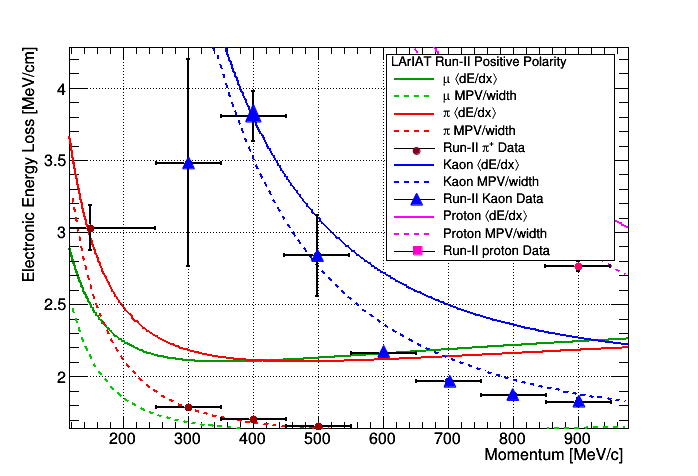
\includegraphics[width=0.48\textwidth]{images/dEdXvsMomentumPosPolRun2Kaon.png}
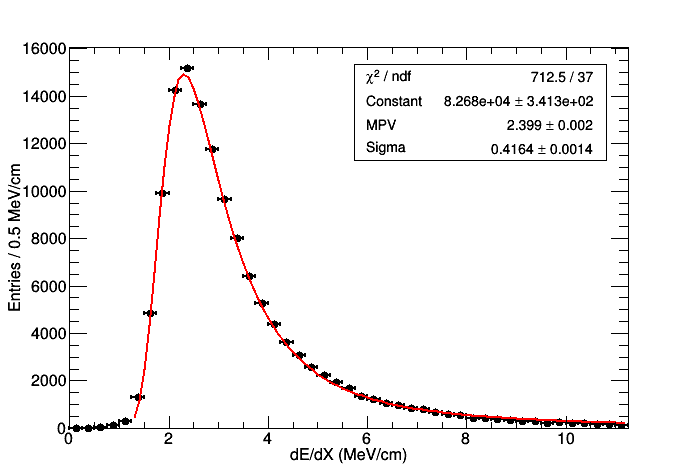
\includegraphics[width=0.48\textwidth]{images/dEdXKaonRunIIPosPol.png}
\caption{(Left) dE/dX vs Momentum for Negative Polarity Picky Tracks: $K^{+}$ sample ,(Right) dE/dX for the entire sample of uniquely matched tracks in the Negative Polarity Picky Tracks: $K^{+}$ sample }
\label{fig:Run2PosPickyTrkKaonResults}
\end{figure}


The distributions here agree relatively well with the theoretical curve. The MPV for the entire $K^{+}$ sample is 2.4 MeV/cm which is slightly higher (as was the case for the other samples) than the expected value of 2.15 MeV/cm for a mean momentum of $\sim$ 724 MeV as shown in Figure \ref{fig:Run2PosPickyTrkKaonMomentumSpec}. 


\begin{figure}[htb]
\centering
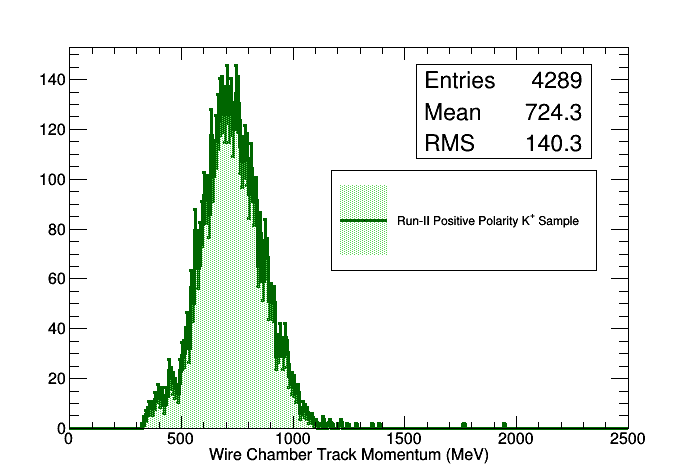
\includegraphics[width=0.55\textwidth]{images/RunIIKaonPosPolWCMomentum.png}
\caption{Wire chamber track momentum spectrum for the Run-II Positive Polarity Picky $K^{+}$ sample  }
\label{fig:Run2PosPickyTrkKaonMomentumSpec}
\end{figure}


In addition to this slight pathology, the lowest momentum bin between 250 MeV and 350 MeV has fluctuated low. This is driven by the fact that the number of entries in this bin is sparse and the fits are not optimal. While the statistics were sufficient to not be excluded outright, this bin should be taken with a pinch of salt.

%%%%%%%%%%%%%%%%%%%%%%%%%%%%%%%%%%%%%%%%%%%%%%%%%%%%%%%
\subsubsection{Positive Polarity Picky Tracks: Proton}\label{sec:Run2PosPickyTrkProton}
%%%%%%%%%%%%%%%%%%%%%%%%%%%%%%%%%%%%%%%%%%%%%%%%%%%%%%%

Using the sample of 36,278 protons selected from the positive polarity picky track sample using the mass cut described in Section \ref{sec:EventSelection} allows for a high dE/dX check of the calibration constants derived in Section \ref{sec:Run2PosPickyTrkPiMuE}. The outcome of the calibration sample is shown in Figure \ref{fig:Run2PosPickyTrkProtonResults}.

\begin{figure}[htb]
\centering
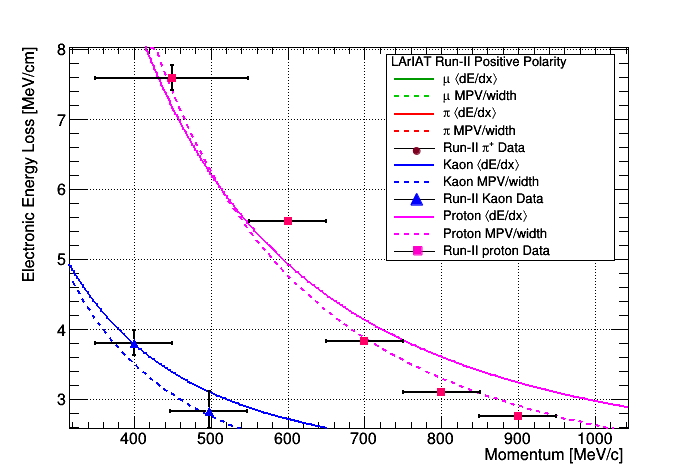
\includegraphics[width=0.48\textwidth]{images/dEdXvsMomentumPosPolRun2ProtonFineBin.png}
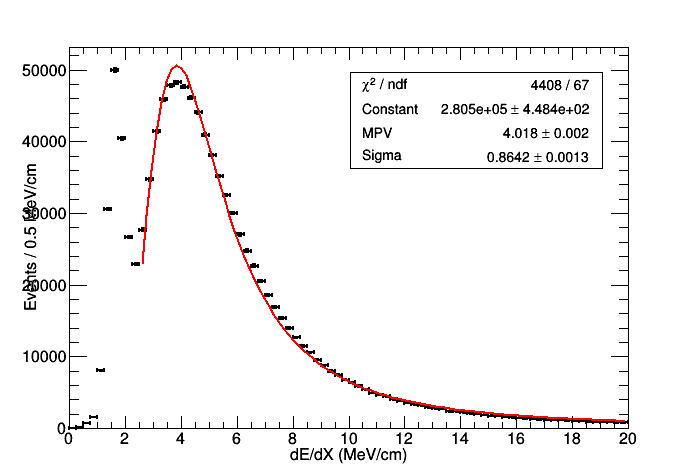
\includegraphics[width=0.48\textwidth]{images/dEdXPosPolRun2Proton.png}
\caption{(Left) dE/dX vs Momentum for Positive Polarity Picky Tracks proton sample ,(Right) dE/dX for the entire sample of uniquely matched tracks in the Positive Polarity Picky Tracks proton sample.}
\label{fig:Run2PosPickyTrkProtonResults}
\end{figure}

Just as before, this sample differs slightly from the $\pi, \mu, e$ samples in that the ranges for the fits have been modified to exclude a contamination coming from minimum ionizing particles. This contamination can be seen in the RHS of Figure \ref{fig:Run2PosPickyTrkProtonResults} with the peak below 2~MeV/cm. Secondly, events with very low statistics in the momentum bins below 350~MeV are excluded from the LHS of Figure \ref{figRun1PosPickyTrkProtonResults} and the lowest bin is merged between 350 MeV and 550 MeV.

The MPV for the entire sample of 4.62 MeV/cm is higher than expected value of 3.85 MeV/cm for a mean momentum of $\sim$725  MeV as was present for this sample, shown in Figure \ref{fig:Run1PosPickyTrkProtonMomentumSpec}. Again, the data points follow the expected Bethe-Bloch behavior rather well despite this disagreement with the mean momentum expectation.

\begin{figure}[htb]
\centering
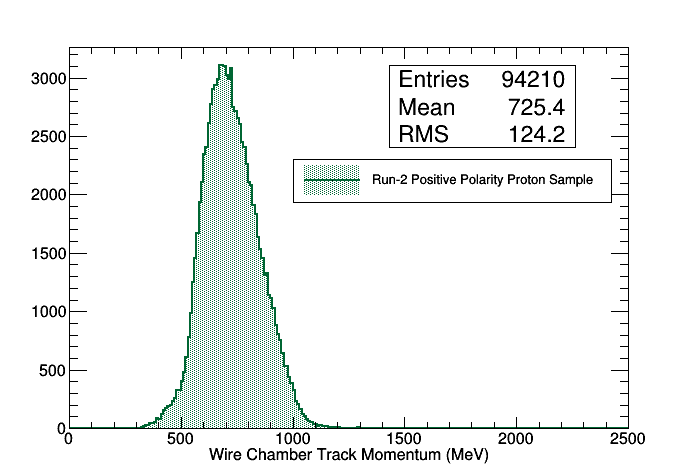
\includegraphics[width=0.55\textwidth]{images/WCTrkMomentumRun2PosProton.png}
\caption{Wire chamber track momentum spectrum for the Run-II Positive Polarity Picky Tracks proton sample  }
\label{fig:Run1PosPickyTrkProtonMomentumSpec}
\end{figure}

\clearpage

%%%%%%%%%%%%%%%%%%%%%%%%%%%%%%%%%%%%%%%%%%%%%%%%%%%%%%%
\subsubsection{Negative Polarity Picky Tracks: $\pi^{-}, \mu^{-}, e^{-}$}\label{sec:Run2NegPickyTrkPiMuE}
%%%%%%%%%%%%%%%%%%%%%%%%%%%%%%%%%%%%%%%%%%%%%%%%%%%%%%%

Using the same calibration constants derived in Section \ref{sec:Run2PosPickyTrkPiMuE}, Figure \ref{fig:Run2NegPickyTrkPiMuEResults} shows the outcome for the sample of 48,976 negative polarity $\pi^{-}, \mu^{-}, e^{-}$ events in Run-II. This sample is used to cross-check the calibration constants derived for the positive polarity sample.

\begin{figure}[htb]
\centering
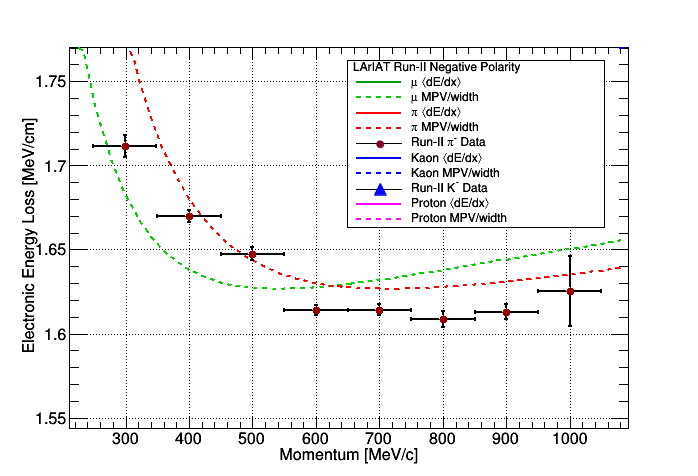
\includegraphics[width=0.48\textwidth]{images/dEdXvsMomentumNegPolRun2FineBin.png}
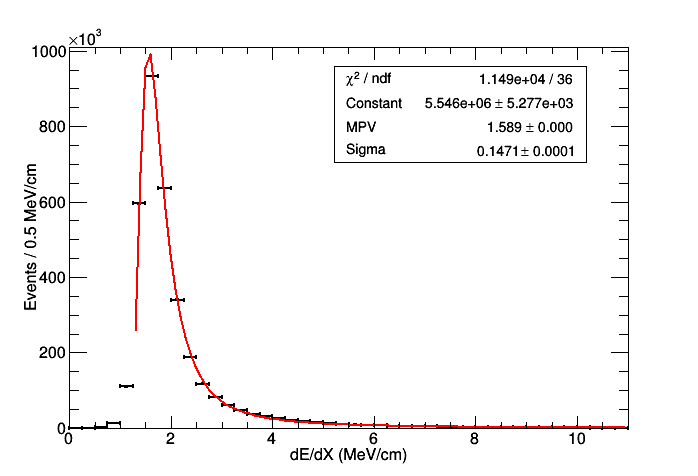
\includegraphics[width=0.48\textwidth]{images/dEdXNegPolRun2.png}
\caption{(Left) dE/dX vs Momentum for Negative Polarity Picky $\pi^{-}, \mu^{-}, e^{-}$ sample ,(Right) dE/dX for the entire sample of uniquely matched tracks in the Negative Polarity Picky Tracks: $\pi^{-}, \mu^{-}, e^{-}$ sample }
\label{fig:Run2NegPickyTrkPiMuEResults}
\end{figure}

The distributions here also agree with the theoretical curve for a sample of pions and muons (as there is expected to be a small contamination of the pion beam with through going muons. The MPV for the entire sample of 1.727 MeV/cm is slightly above the expected value of 1.65 MeV/cm for a mean momentum of $\sim$500 MeV as was present for this sample, shown in Figure \ref{fig:Run2NegPickyTrkPiMuEMomentumSpec}.

\begin{figure}[htb]
\centering
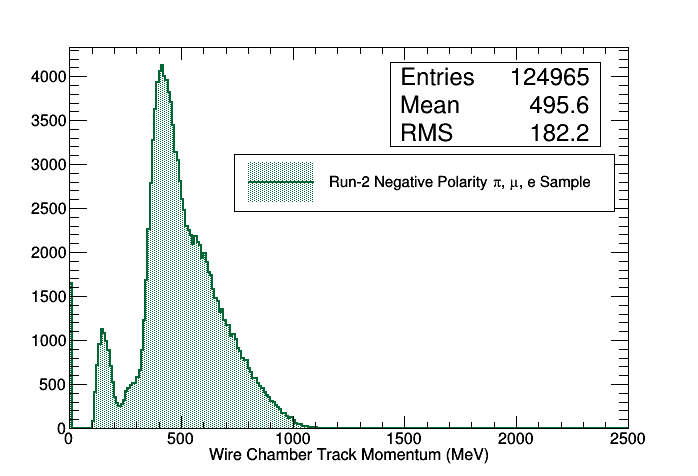
\includegraphics[width=0.55\textwidth]{images/WCTrkMomentumRun2NegPiMuE.png}
\caption{Wire chamber track momentum spectrum for the Run-II Negative Polarity Picky Tracks $\pi, \mu, e$ sample  }
\label{fig:Run2NegPickyTrkPiMuEMomentumSpec}
\end{figure}


%%%%%%%%%%%%%%%%%%%%%%%%%%%%%%%%%%%%%%%%%%%%%%%%%%%%%%%
\subsubsection{Negative Polarity Picky Tracks: $K^{-}$}\label{sec:Run2NegPickyTrkKaonMinus}
%%%%%%%%%%%%%%%%%%%%%%%%%%%%%%%%%%%%%%%%%%%%%%%%%%%%%%%
The sample of 215 negative polarity $K^{-}$ picky track events present in Run-II provide a final check the calibration constants provided in Section \ref{sec:Run2PosPickyTrkPiMuE}. This samples very small statistics limits the overall usefulness of this cross-check, but is provided here for completeness.

Figure \ref{fig:Run2NegPickyTrkKaonResults} shows the dE/dX vs momentum and the aggregate dE/dX distribution obtained with these calorimetry constants.

\begin{figure}[htb]
\centering
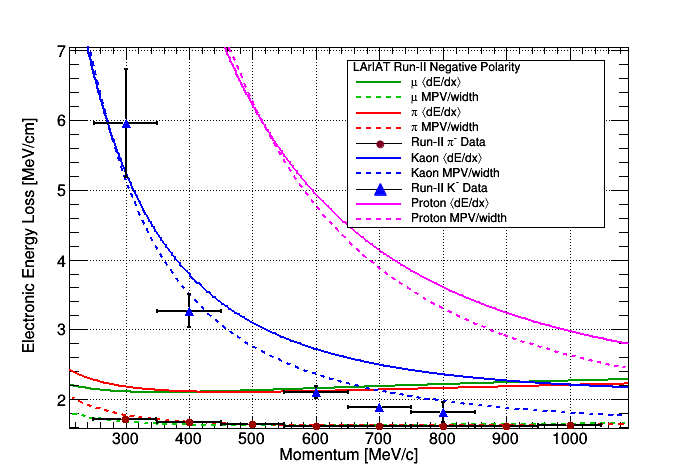
\includegraphics[width=0.48\textwidth]{images/dEdXvsMomentumNegPolRun2Kaon.png}
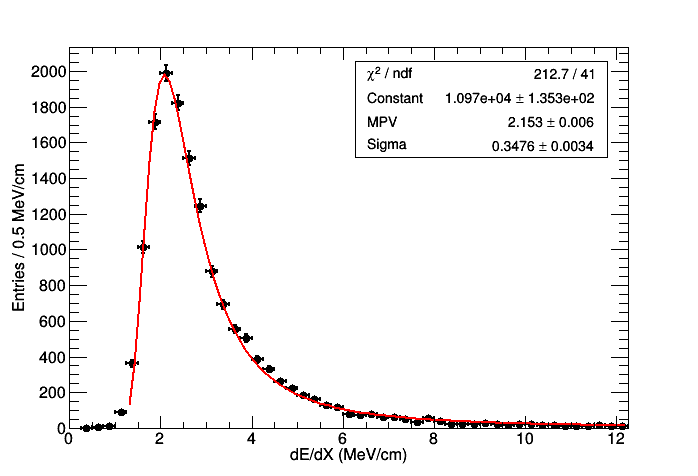
\includegraphics[width=0.48\textwidth]{images/dEdXKaonRunIINegPol.png}
\caption{(Left) dE/dX vs Momentum for Negative Polarity Picky Tracks: $K^{-}$ sample ,(Right) dE/dX for the entire sample of uniquely matched tracks in the Negative Polarity Picky Tracks: $K^{-}$ sample }
\label{fig:Run2NegPickyTrkKaonResults}
\end{figure}

%%%%%%%%%%%%%%%%%%%%%%%%%%%%%%%%%%%%%%%%%%%%%%%%%%%%%%%
\subsection{Run-I Cosmic Data}\label{sec:RunICosmics}
%%%%%%%%%%%%%%%%%%%%%%%%%%%%%%%%%%%%%%%%%%%%%%%%%%%%%%%

As a last check for the calorimetry constants derived, a sample of through going cosmic ray events are selected from a subsample of negative polarity Run-I data. These events are chosen because they have significantly different angle and energy than the beamline tracks used thus far to tune the calorimetry constant.

The selection criteria for these events is: 

\begin{itemize}
\item \textbf{Cosmic Time-Stamp Event}:

\begin{verbatim}
tfilt:      @local::lariat_timestampfilter

# ====================================================================
# Specify range of events to select.  For Run I/II:
#   - pedestal events:  ~ 0.  - 1.2 sec
#   - beam events:      ~ 1.2 - 5.5 sec
#   - cosmic events:    ~ > 5.5 sec
#   (default selects ALL events)
physics.filters.tfilt.T1:                       7.5
physics.filters.tfilt.T2:                       40
physics.filters.tfilt.RequireRawDigits:         true

\end{verbatim}

For this sample, a $T_{1}$ start time of 7.5 seconds was chosen to ensure no contamination from beam events would be present in the TPC prior to receiving a cosmic trigger.


\item \textbf{Single Track Reconstructed}:

Next we require one and only one track reconstructed inside the TPC to avoid any confusion with the track which is being analyzed.

\item \textbf{Vertical Track Requirement}

To help ensure these events have a very different topology than the ones used in the initial calibration, we require the track to have traversed at least 35~cm in the $y$ direction. This ensures the tracks are of high energy and in general vertical going.

\end{itemize}

For Run-I negative polarity data (using the magnet current only to define the data taking period) this selects 59,991 events. Figure \ref{fig:CosmicDist} shows the $y$ vs $z$ distribution of the 3-d points which make up the tracks in the cosmic sample and the dE/dX vs residual range for these tracks. This illustrates that the majority of the tracks traverse the vertical distance of the TPC, while some do manage to traverse a much more diagonal distance. This sample also samples all parts of the TPC fairly uniformly, allowing us to check the calibration in different portions of the TPC.

\begin{figure}[htb]
\centering
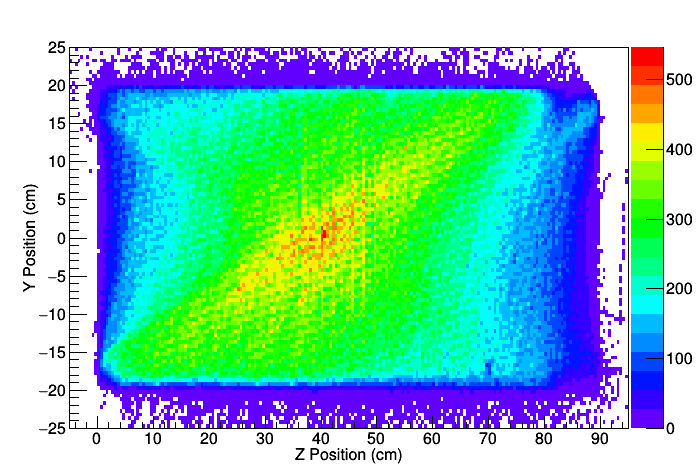
\includegraphics[width=0.45\textwidth]{images/CosmicDistYZ.png}
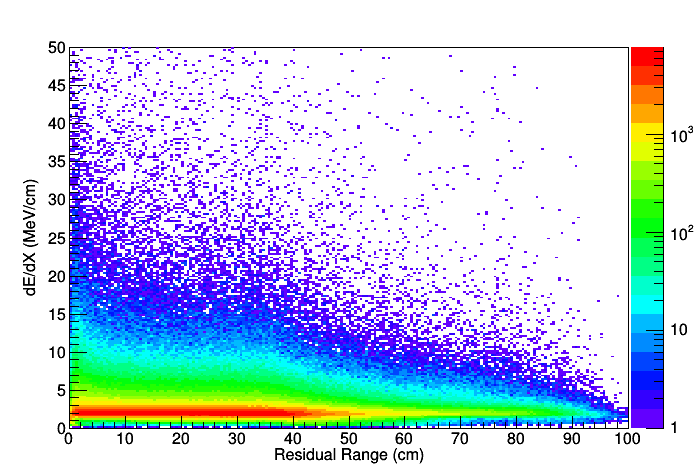
\includegraphics[width=0.45\textwidth]{images/CosmicDistdEdXRR.png}
\caption{(Left) The y vs x position of all the 3-d points which make up the sample of cosmics used for this sample ,(Right) dE/dX vs Residual Range (RR) for the sample of cosmics demonstrating the range of the sample going from 40 cm up to the full diagonal distance of the TPC.}
\label{fig:CosmicDist}
\end{figure}


Figure \ref{fig:CosmicdEdX} shows the dE/dX distribution for this sample of 59,991 events fit with a Landau. This returns a MPV of 1.7 MeV/cm. When compared to the expected value for cosmic ray muons with a momentum of $\sim$5~GeV (as is expected for muons going through LArIAt at sea level) we would expect to get a MPV of 1.73 MeV/cm. Thus our previously derived calibration constants do reproduce the expected distribution for a sample of cosmic rays.

\begin{figure}[htb]
\centering
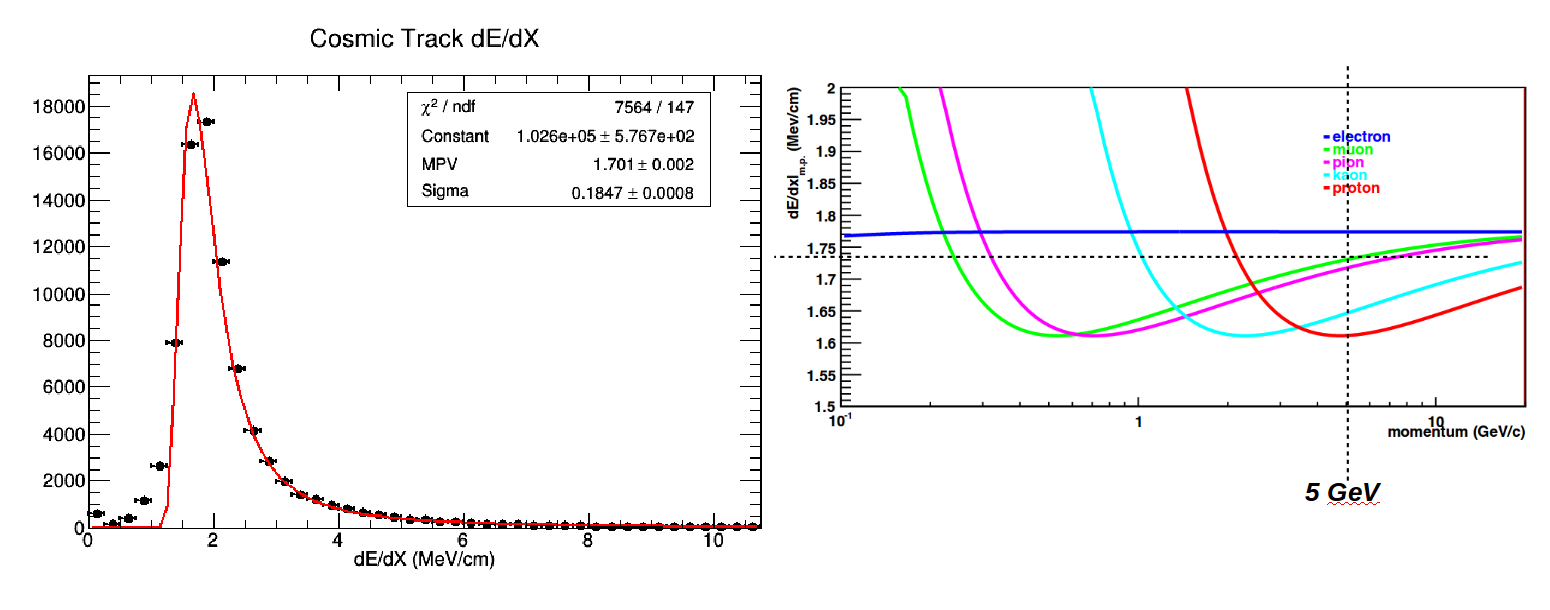
\includegraphics[width=0.45\textwidth]{images/CosmicdEdX.png}
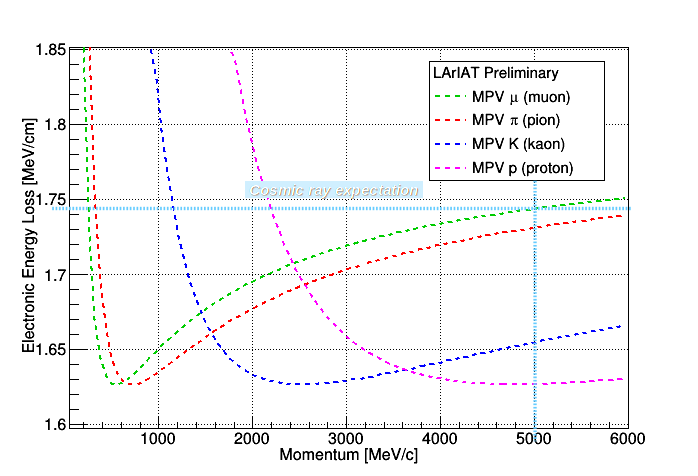
\includegraphics[width=0.45\textwidth]{images/CosmicRayExpectation.png}
\caption{(Left) The dE/dX distribution for the sample of Cosmic tracks fit with a Landau function giving a MPV of 1.7 MeV/cm. ,(Right) The theoretical prediction for cosmic ray muons with a mean momentum of $\sim$5~GeV would return a dE/dX MPV of 1.75 MeV/cm.}
\label{fig:CosmicdEdX}
\end{figure}

Finally, Figure \ref{fig:CosmicdEdXSections} shows the dE/dX distribution if you restrict to only looking at specific portions of the TPC in the $z$ direction. We divide the TPC into four equal portions in $z$ and see the dE/dX response is nearly uniform with the MPV varying 0.094 from the lowest to highest value. 

\begin{figure}[htb]
\centering
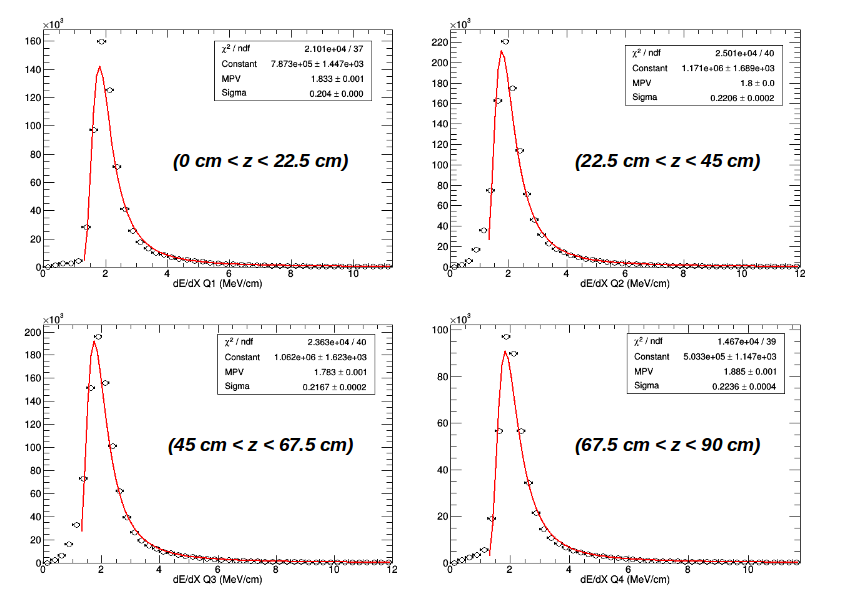
\includegraphics[width=0.95\textwidth]{images/CosmicFourSections.png}
\caption{dE/dX distribution over the four sections of the TPC as divided in $z$ from our cosmic data sample.}
\label{fig:CosmicdEdXSections}
\end{figure}



\clearpage

%%%%%%%%%%%%%%%%%%%%%%%%%%%%%%%%%%%%%%%%%%%%%%%%%%%%%%%
\subsection{Monte Carlo}\label{sec:MCResults}
%%%%%%%%%%%%%%%%%%%%%%%%%%%%%%%%%%%%%%%%%%%%%%%%%%%%%%%

Finally, a similar procedure is used to tune the Monte Carlo dE/dX response. For the purposes of the note a sample of data driven Monte Carlo (DDMC) using the Run-I momentum profile  for a sample of pions and protons is chosen. The Monte Carlo pion sample is used to tune the constants and then this is checked with Monte Carlo protons. Since only the momentum spectrum changes between Run-I and Run-II MC, this tuning should be sufficient to be applied to all the MC samples used. Table \ref{tab:MCCutSummary} summarizes the event selection used for these MC samples.

\begin{table}[htb]
	\begin{center}
	\resizebox{0.95\textwidth}{!}{%
	\begin{tabular}{|c|c|c|}
	\hline
	%\multicolumn{5}{|c|}{\textbf{Summary of inclusive NC $\pi^{0}$ Event Selection Cuts}} \\
	%\hline \hline
	  \textbf{Event Selection} & Run-I Negative Polarity & Run-I Positive Polarity   \\
	   & Pion-MC & Proton MC  \\
	\hline
	Total Number of Events & 265,000  & 320,000 \\
	\hline
	MC Particle reaches the TPC & 196,262  & 256,256 \\
	\hline
	Unique match between MC and TPC Track & 148,002  & 224,982  \\
	\hline
	\hline
	\end{tabular}}
	\caption{Summary of Monte Carlo event selection applied to the calibration sample.} \label{tab:MCCutSummary}
	\end{center}
\end{table}

%%%%%%%%%%%%%%%%%%%%%%%%%%%%%%%%%%%%%%%%%%%%%%%%%%%%%%%
\subsubsection{Pion MC}\label{sec:Pion MC}
%%%%%%%%%%%%%%%%%%%%%%%%%%%%%%%%%%%%%%%%%%%%%%%%%%%%%%%

For the DDMC samples we correct from MC-truth the energy the pions lose in the upstream portion of the detector between where they are launched ($z=-100$~cm) and the front face of the TPC. This correction is applied on a particle by particle basis, thus the momentum used in the calibration is the true momentum the proton has in the first 5~cm of the TPC.

Calibration constants for this sample are \verb!physics.producers.calo.CaloAlg.CalAreaConstants: [0.094, 0.101]! and the results of this are plotted on Figure \ref{fig:DDMCPionResults}. One peculiar feature still under investigation is the lack of relativistic rise in the region above 500 MeV. These constants were decided upon because they give a MPV for the overall dE/dX distribution which agrees well with the value found in the data for Run-I from Section \ref{sec:Run1NegPickyTrkPiMuE}.

\begin{figure}[htb]
\centering
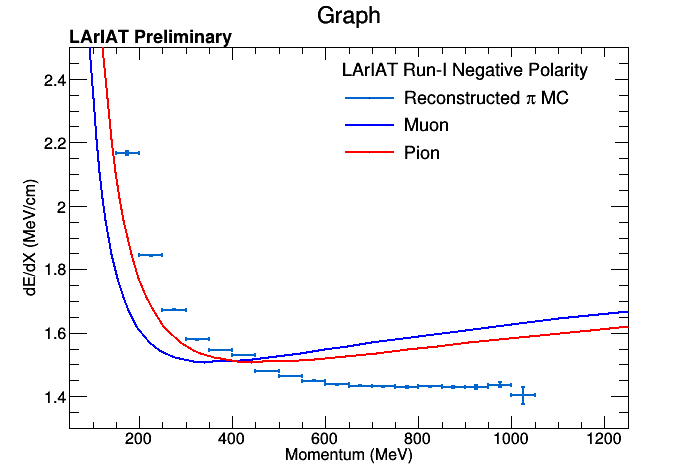
\includegraphics[width=0.48\textwidth]{images/dEdXvsMomentumPionMCVeryFineBin.png}
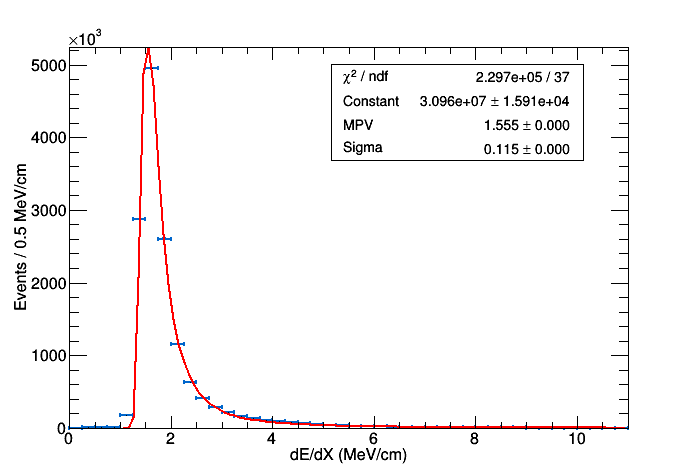
\includegraphics[width=0.48\textwidth]{images/dEdXDDMCPionRunI.png}
\caption{(Left) dE/dX vs Momentum for Data Driven Pion MC using Run-I negative polarity momentum spectrum ,(Right) dE/dX for the entire sample of uniquely matched tracks in the DDMC pion sample.}
\label{fig:DDMCPionResults}
\end{figure}

We check this tuning using a sample of protons in the next section.

%%%%%%%%%%%%%%%%%%%%%%%%%%%%%%%%%%%%%%%%%%%%%%%%%%%%%%%
\subsubsection{Proton MC}\label{sec:Proton MC}
%%%%%%%%%%%%%%%%%%%%%%%%%%%%%%%%%%%%%%%%%%%%%%%%%%%%%%%

For the DDMC samples we correct from MC-truth the energy the protons lose in the upstream portion of the detector between where they are launched ($z=-100$~cm) and the front face of the TPC. This correction is applied on a particle by particle basis, thus the momentum used in the calibration is the true momentum the proton has in the first 5cm of the TPC.

Figure \ref{fig:DDMCProtonResults} shows the results of applying the calibration constants derived in Section \ref{sec:Pion MC} to the sample of protons. Very good agreement is seen across the majority of the momentum spectrum.

\begin{figure}[htb]
\centering
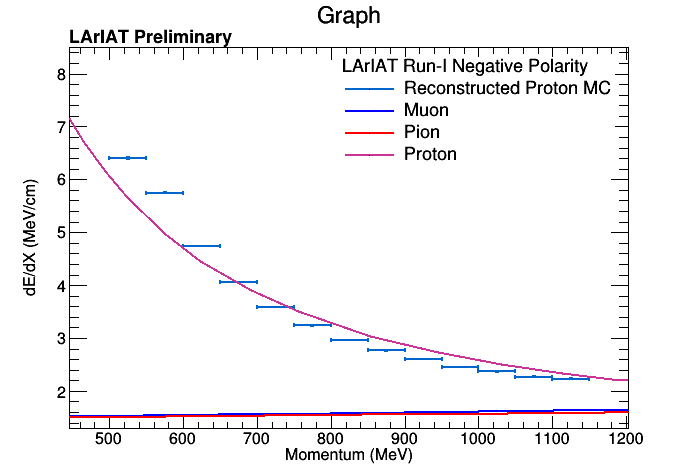
\includegraphics[width=0.48\textwidth]{images/dEdXvsMomentumProtonMCVeryFineBin.png}
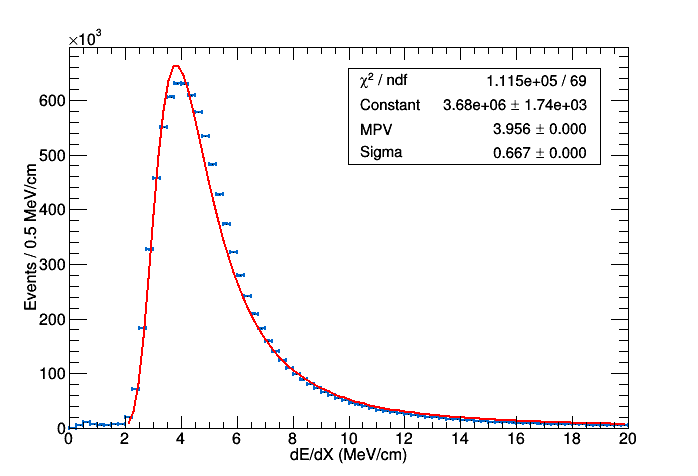
\includegraphics[width=0.48\textwidth]{images/dEdXDDMCProtonRunI.png}
\caption{(Left) dE/dX vs Momentum for Data Driven Proton MC using Run-I positive polarity momentum spectrum ,(Right) dE/dX for the entire sample of uniquely matched tracks in the DDMC Proton sample.}
\label{fig:DDMCProtonResults}
\end{figure}


The MPV for the DDMC proton sample is found to be 3.956 MeV/cm. This result is consistent with the data value of 3.902 MeV/cm obtained from Run-I positive polarity picky track sample in Seciton \ref{sec:Run1PosPickyTrkProton}. The MC is absent the contamination seen in the data and thus does not have the peak in the dE/dX spectrum seen in the data below 2 MeV/cm.


These calorimetry constants will be used for all the Data Driven Monte Carlo produced for the forthcoming inclusive cross-section analyses.
\newpage





\newpage
\section{Results}\label{sec:Results}


%%%%%%%%%%%%%%%%%%%%%%%%%%%%%%%%%%%%%%%%%%%%%%%%%%%%%%%
\subsection{Run-I Data}\label{sec:RunI}
%%%%%%%%%%%%%%%%%%%%%%%%%%%%%%%%%%%%%%%%%%%%%%%%%%%%%%%
Table \ref{tab:RunICutSummary} summarizes the number of events which are selected to use as the calibration or validation samples in order to tune our calorimetry constants.

%%% Put event reduction tables here 
\begin{table}[htb]
	\begin{center}
	\resizebox{0.98\textwidth}{!}{%
	\begin{tabular}{|c|c|c|c|c|c|}
	\hline
	%\multicolumn{5}{|c|}{\textbf{Summary of inclusive NC $\pi^{0}$ Event Selection Cuts}} \\
	%\hline \hline
	  \textbf{Event Selection} & Run-I Negative Polarity & Run-I Negative Polarity &  Run-I Positive Polarity & Run-I Positive Polarity & Run-I Positive Polarity  \\
	   & $\pi^{-}, \mu^{-}, e^{-}$ & $K^{-}$ & $\pi^{+}, \mu^{+}, e^{+}$ & $K^{+}$ & Proton  \\
	\hline
	Beam Filter & 113,042 & 113,042 & 140,954 & 140,954 & 140,954 \\
	\hline
	Mass Selection & 5,909 & 63 & 5,349 & 346 &  9,104 \\
	\hline
	$>$ 1 Track Reconstructed in the TPC & 5,722  & 58 & 5,223 & 337  & 8,062  \\
	\hline
	$<$ 3 Tracks Reconstructed &  &  &  &  &  \\
	with length $<$ 5~cm & 4,323 & 45 & 4,058 &  263 & 6,561  \\
	\hline
	Unique match between WC and TPC Track & 2,464 & 17 & 2,446  & 120 & 3,373  \\
	\hline
	\hline
	\end{tabular}}
	\caption{Summary of event selection applied to the calibration sample for Run-I data.} \label{tab:RunICutSummary}
	\end{center}
\end{table}

Figure \ref{fig:Run1NegPosPickyTrkTotal} shows the total calibration for Run-I data samples using the calorimetry constants \verb!physics.producers.calo.CaloAlg.CalAreaConstants: [0.025,0.052]!. The results only show the tuning of the collection plane values. Due to the limited statistics in the kaon sample, bins in momentum with too few entries were omitted from the plot due to the poor fit values returned. 

In the sub-sections below we focus in on the various sub-samples to show the results of the tuning in detail.

\begin{figure}[h!]
\centering
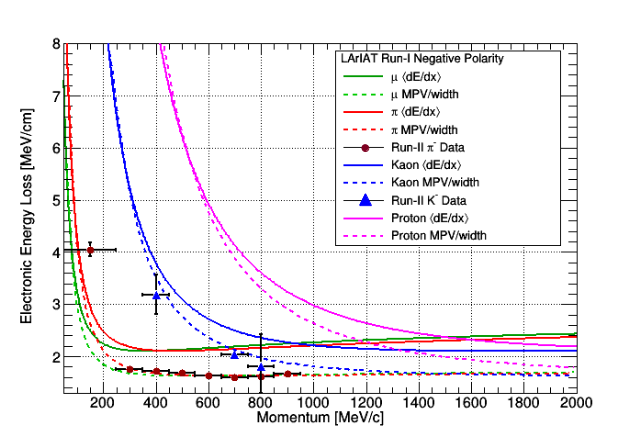
\includegraphics[width=0.75\textwidth]{images/RunINegTotaldEdXvsMomentum.png}
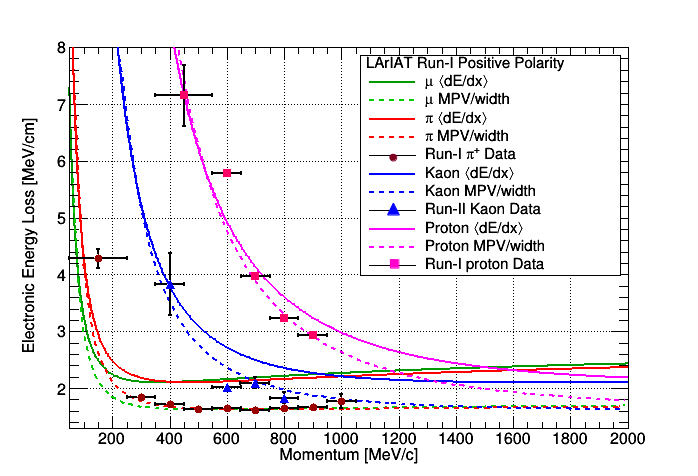
\includegraphics[width=0.75\textwidth]{images/RunIPosTotaldEdXvsMomentum.png}
\caption{(Left) dE/dX vs Momentum for Run-I Negative Polarity Picky Tracks: $\pi^{-}, \mu^{-}, e^{-}$ and $K^{-}$ sample ,(Right) dE/dX vs Momentum for Run-I Positive Polarity Picky Tracks: $\pi^{+}, \mu^{+}, e^{+}$ and $K^{+}$, and Proton sample. }
\label{fig:Run1NegPosPickyTrkTotal}
\end{figure}

\clearpage

%%%%%%%%%%%%%%%%%%%%%%%%%%%%%%%%%%%%%%%%%%%%%%%%%%%%%%%
\subsubsection{Negative Polarity Picky Tracks: $\pi^{-}, \mu^{-}, e^{-}$}\label{sec:Run1NegPickyTrkPiMuE}
%%%%%%%%%%%%%%%%%%%%%%%%%%%%%%%%%%%%%%%%%%%%%%%%%%%%%%%

The sample of 2,464 negative polarity $\pi^{-}, \mu^{-}, e^{-}$ picky tracks was used to tune the calorimetry constants for Run-I. After several iterations the calo constants \verb!physics.producers.calo.CaloAlg.CalAreaConstants: [0.025,0.052]! were chosen. Figure \ref{fig:Run1NegPickyTrkPiMuEResults} shows the dE/dX vs momentum and the aggregate dE/dX distribution obtained with these calorimetry constants.

\begin{figure}[htb]
\centering
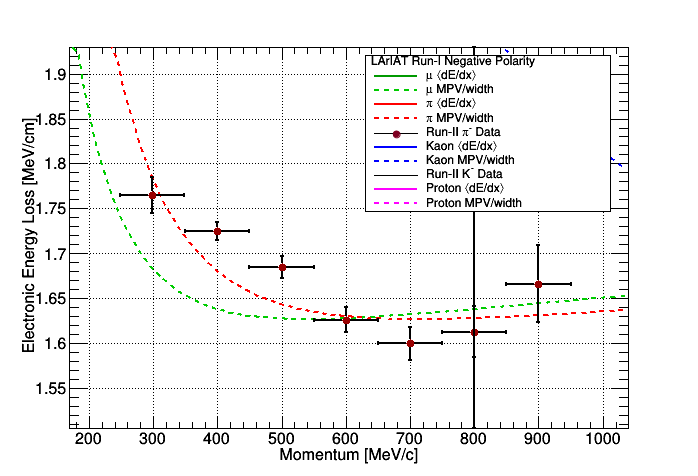
\includegraphics[width=0.48\textwidth]{images/dEdXvsMomentumNegPolRun1FineBin2.png}
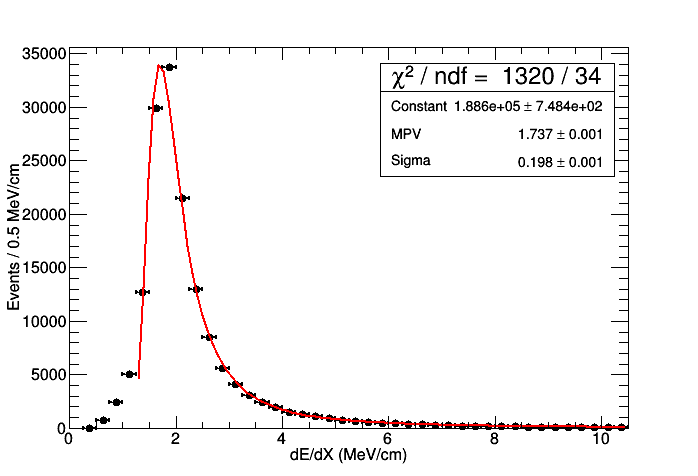
\includegraphics[width=0.48\textwidth]{images/dEdXRun1NegPolFinal.png}
\caption{(Top) dE/dX vs Momentum for Negative Polarity Picky Tracks: $\pi^{-}, \mu^{-}, e^{-}$ sample ,(Bottom) dE/dX for the entire sample of uniquely matched tracks in the Negative Polarity Picky Tracks: $\pi^{-}, \mu^{-}, e^{-}$ sample }
\label{fig:Run1NegPickyTrkPiMuEResults}
\end{figure}

The distributions here generally agree with the theoretical curve for a sample of pions and muons (as there is expected to be a small contamination of the pion beam with through going muons. The MPV for the entire sample of 1.737 MeV/cm is slightly higher than the expected value of 1.65 MeV/cm for a mean momentum of $\sim$500 MeV as was present for this sample, shown in Figure \ref{fig:Run1NegPickyTrkPiMuEMomentumSpec}.

\begin{figure}[htb]
\centering
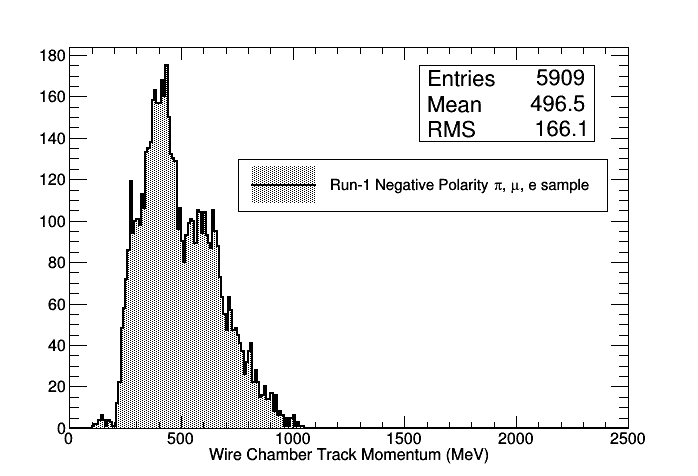
\includegraphics[width=0.55\textwidth]{images/WCTrkMomentumRun1NegPiMuE.png}
\caption{Wire chamber track momentum spectrum for the Run-I Negative Polarity Picky Tracks: $\pi, \mu, e$ sample  }
\label{fig:Run1NegPickyTrkPiMuEMomentumSpec}
\end{figure}

Even with this slight inconsistency between the expected MPV for the mean momentum of the sample and the measured value, these calorimetry constants do provide a good characterization of the overall Bethe-Bloch curve and, as we will see in the other samples, work well for kaons, protons, and positive pions.

%%%%%%%%%%%%%%%%%%%%%%%%%%%%%%%%%%%%%%%%%%%%%%%%%%%%%%%
\subsubsection{Negative Polarity Picky Tracks: $K^{-}$}\label{sec:Run1NegPickyTrkKaonMinus}
%%%%%%%%%%%%%%%%%%%%%%%%%%%%%%%%%%%%%%%%%%%%%%%%%%%%%%%
The sample of 17 negative polarity $K^{-}$ picky track events was used to first check the calibration constants provided in Section \ref{sec:Run1NegPickyTrkPiMuE}. This samples very small statistics limits the overall usefulness of this cross-check, but is provided here for completeness.

Figure \ref{fig:Run1NegPickyTrkKaonResults} shows the dE/dX vs momentum and the aggregate dE/dX distribution obtained with these calorimetry constants.

\begin{figure}[htb]
\centering
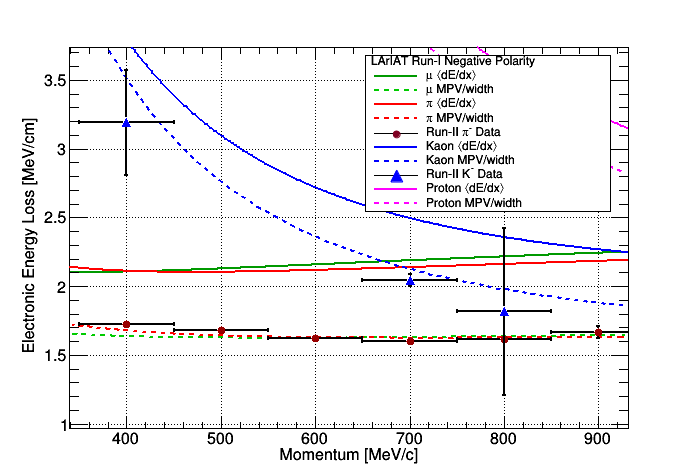
\includegraphics[width=0.48\textwidth]{images/dEdXvsMomentumNegPolRun1Kaon.png}
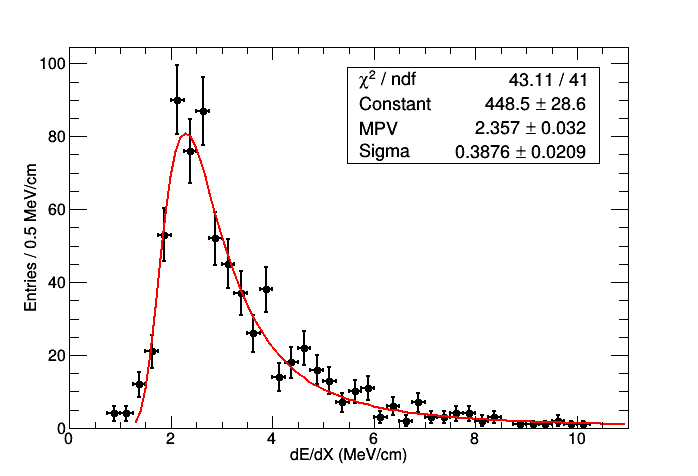
\includegraphics[width=0.48\textwidth]{images/dEdXKaonRunINegPol.png}
\caption{(Left) dE/dX vs Momentum for Negative Polarity Picky Tracks: $K^{-}$ sample ,(Right) dE/dX for the entire sample of uniquely matched tracks in the Negative Polarity Picky Tracks: $K^{-}$ sample }
\label{fig:Run1NegPickyTrkKaonResults}
\end{figure}

%%%%%%%%%%%%%%%%%%%%%%%%%%%%%%%%%%%%%%%%%%%%%%%%%%%%%%%
\subsubsection{Positive Polarity Picky Tracks: $\pi^{+}, \mu^{+}, e^{+}$}\label{sec:Run1PosPickyTrkPiMuE}
%%%%%%%%%%%%%%%%%%%%%%%%%%%%%%%%%%%%%%%%%%%%%%%%%%%%%%%

Using the same calibration constants derived in Section \ref{sec:Run1NegPickyTrkPiMuE}, we now look at the positive polarity sample of data collected in Run-I to validate the constants derived.  Figure \ref{fig:Run1PosPickyTrkPiMuEResults} shows the outcome for the sample of 2,446 positive polarity  $\pi^{+}, \mu^{+}, e^{+}$ events in Run-I.

\begin{figure}[htb]
\centering
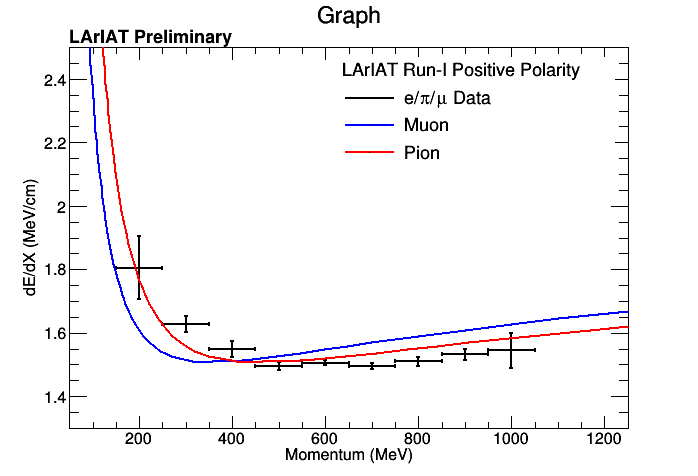
\includegraphics[width=0.48\textwidth]{images/dEdXvsMomentumPosPolRun1FineBin.png}
\includegraphics[width=0.48\textwidth]{images/dEdXPosPolRun1.png}
\caption{(Left) dE/dX vs Momentum for Positive Polarity Picky Tracks: $\pi^{+}, \mu^{+}, e^{+}$ sample ,(Right) dE/dX for the entire sample of uniquely matched tracks in the Positive Polarity Picky Tracks: $\pi^{+}, \mu^{+}, e^{+}$ sample }
\label{fig:Run1PosPickyTrkPiMuEResults}
\end{figure}

The distributions here also agree with the theoretical curve for a sample of pions and muons (as there is expected to be a small contamination of the pion beam with through going muons). The MPV for the entire sample of 1.74 MeV/cm which again is slightly higher than the expected 1.65 MeV/cm for a mean momentum of $\sim$650 MeV as was present for this sample, shown in Figure \ref{fig:Run1PosPickyTrkPiMuEMomentumSpec}. Despite this, teh data follows the Bethe-Bloch curve relatively well and validates the calibration constants derived with an independent sample of pions.

\begin{figure}[htb]
\centering
\includegraphics[width=0.55\textwidth]{images/WCTrkMomentumRun1PosPiMuE.png}
\caption{Wire chamber track momentum spectrum for the Run-I Positive Polarity Picky Tracks: $\pi, \mu, e$ sample}
\label{fig:Run1PosPickyTrkPiMuEMomentumSpec}
\end{figure}

%%%%%%%%%%%%%%%%%%%%%%%%%%%%%%%%%%%%%%%%%%%%%%%%%%%%%%%
\subsubsection{Positive Polarity Picky Tracks: $K^{+}$}\label{sec:Run1PosPickyTrkKaons}
%%%%%%%%%%%%%%%%%%%%%%%%%%%%%%%%%%%%%%%%%%%%%%%%%%%%%%%
The sample of 120 positive polarity $K^{+}$ picky track events was used to check the calibration constants provided in Section \ref{sec:Run1NegPickyTrkPiMuE}. This samples small statistics limits the overall usefulness of this cross-check, but is provided here for completeness.

Figure \ref{fig:Run1PosPickyTrkKaonResults} shows the dE/dX vs momentum and the aggregate dE/dX distribution obtained with these calorimetry constants.

\begin{figure}[htb]
\centering
\includegraphics[width=0.48\textwidth]{images/dEdXvsMomentumPosPolRun1Kaon.png}
\includegraphics[width=0.48\textwidth]{images/dEdXKaonRunIPosPol.png}
\caption{(Left) dE/dX vs Momentum for Negative Polarity Picky Tracks: $K^{+}$ sample ,(Right) dE/dX for the entire sample of uniquely matched tracks in the Negative Polarity Picky Tracks: $K^{+}$ sample }
\label{fig:Run1PosPickyTrkKaonResults}
\end{figure}


%%%%%%%%%%%%%%%%%%%%%%%%%%%%%%%%%%%%%%%%%%%%%%%%%%%%%%%
\subsubsection{Positive Polarity Picky Tracks: Proton}\label{sec:Run1PosPickyTrkProton}
%%%%%%%%%%%%%%%%%%%%%%%%%%%%%%%%%%%%%%%%%%%%%%%%%%%%%%%

As a final cross-check for Run-1, a sample of protons is selected from the positive polarity picky track sample using the mass cut described in Section \ref{sec:EventSelection} using the same calibration constants derived in Section \ref{sec:Run1NegPickyTrkPiMuE}. The outcome of the calibration sample is shown in Figure \ref{fig:Run1PosPickyTrkProtonResults}.

\begin{figure}[htb]
\centering
\includegraphics[width=0.48\textwidth]{images/dEdXvsMomentumPosPolRun1ProtonFineBin.png}
\includegraphics[width=0.48\textwidth]{images/dEdXPosPolRun1Proton.png}
\caption{(Left) dE/dX vs Momentum for Positive Polarity Picky Tracks proton sample ,(Right) dE/dX for the entire sample of uniquely matched tracks in the Positive Polarity Picky Tracks proton sample.}
\label{fig:Run1PosPickyTrkProtonResults}
\end{figure}

This sample differs slightly from the $\pi^{+}, \mu^{+}, e^{+}$ samples in that the ranges for the fits have been modified to exclude a contamination coming from minimum ionizing particles. This contamination can be seen in the RHS of Figure \ref{fig:Run1PosPickyTrkProtonResults} with the peak below 2~MeV/cm. Secondly, events with very low statistics in the momentum bins below 350~MeV are excluded from the LHS of Figure \ref{fig:Run1PosPickyTrkProtonResults} and the lowest bin is merged between 350 MeV and 550 MeV.

The MPV for the entire sample of 4.55 MeV/cm is slightly above expected value of 3.9 MeV/cm for a mean momentum of $\sim$730 MeV as was present for this sample, shown in Figure \ref{fig:Run1PosPickyTrkProtonMomentumSpec}. This slightly higher MPV is consistent with the results seen in the $\pi, \mu, e$ samples, but overall the data follows the Bethe-Bloch curve relatively well.

\begin{figure}[htb]
\centering
\includegraphics[width=0.55\textwidth]{images/WCTrkMomentumRun1PosProton.png}
\caption{Wire chamber track momentum spectrum for the Run-I Positive Polarity Picky Tracks proton sample  }
\label{fig:Run1PosPickyTrkProtonMomentumSpec}
\end{figure}

The overall agreement for these five samples using the calorimetry constants derived for Run-I validate the procedure and we now shift our attention to the applying the same methodology to Run-II data.

\newpage
%%%%%%%%%%%%%%%%%%%%%%%%%%%%%%%%%%%%%%%%%%%%%%%%%%%%%%%
\subsection{Run-II Data}\label{sec:RunII}
%%%%%%%%%%%%%%%%%%%%%%%%%%%%%%%%%%%%%%%%%%%%%%%%%%%%%%%
Table \ref{tab:RunIICutSummary} summarizes the number of events which are selected to use as the calibration or validation samples in order to tune our calorimetry constants for Run-II.

%%% Put event reduction tables here 
\begin{table}[htb]
	\begin{center}
	\resizebox{0.95\textwidth}{!}{%
	\begin{tabular}{|c|c|c|c|c|c|}
	\hline
	%\multicolumn{5}{|c|}{\textbf{Summary of inclusive NC $\pi^{0}$ Event Selection Cuts}} \\
	%\hline \hline
	  \textbf{Event Selection} & Run-II Negative Polarity & Run-II Negative Polarity  & Run-II Positive Polarity & Run-II Positive Polarity & Run-II Positive Polarity  \\
	   & $\pi^{-}, \mu^{-}, e^{-}$ & $K^{-}$ & $\pi^{+}, \mu^{+}, e^{+}$ & $K^{+}$ & Proton  \\
	\hline
	Beam Filter & 1,585,598 & 1,585,598  & 1,555,402 & 1,555,402  & 1,555,402 \\
	\hline
	Mass Selection & 124,965 & 835 & 89,561 & 4,289 & 94,210 \\
	\hline
	$>$ 1 Track Reconstructed in the TPC & 117,869 & 601 & 86,918 & 4,083 & 82,099  \\
	\hline
	$<$ 3 Tracks Reconstructed &  &  &  &  &  \\
	with length $<$ 5~cm & 88,717 & 428 & 69,509 & 3,385 & 68,847  \\
	\hline
	Unique match between WC and TPC Track & 48,076  & 216 & 43,547 & 1,719 & 36,278  \\
	\hline
	\hline
	\end{tabular}}
	\caption{Summary of event selection applied to the calibration sample.} \label{tab:RunIICutSummary}
	\end{center}
\end{table}

Figure \ref{fig:Run2NegPosPickyTrkTotal} shows the total calibration for Run-II data samples using the calorimetry constants \verb!physics.producers.calo.CaloAlg.CalAreaConstants: [0.022,0.0445]!. The results only show the tuning of the collection plane values. Due to the limited statistics in the kaon sample, bins in momentum with too few entries were omitted from the plot due to the poor fit values returned. 

\begin{figure}[h!]
\centering
\includegraphics[width=0.75\textwidth]{images/RunIINegTotaldEdXvsMomentum.png}
\includegraphics[width=0.75\textwidth]{images/RunIIPosTotaldEdXvsMomentum.png}
\caption{(Top) dE/dX vs Momentum for Run-II Negative Polarity Picky Tracks: $\pi^{-}, \mu^{-}, e^{-}$ and $K^{-}$ sample ,(Bottom) dE/dX vs Momentum for Run-II Positive Polarity Picky Tracks: $\pi^{+}, \mu^{+}, e^{+}$ and $K^{+}$, and Proton sample. }
\label{fig:Run2NegPosPickyTrkTotal}
\end{figure}

For Run-II data, a slightly different order was followed in tuning the calibration constants. For this set of data we began with positive polarity picky tracks  $\pi^{+}, \mu^{+}, e^{+}$ sample and then checked this tuning with $K^{+}$ and the proton sample before cross-checking with the negative polarity picky tracks  $\pi^{-}, \mu^{-}, e^{-}$ and $K^{-}$ sample. This was done to help ensure the samples weren't being biased in the tuning for the negative polarity pion inclusive cross-section sample.  The order is the method was applied is represented by the section numbering.

%%%%%%%%%%%%%%%%%%%%%%%%%%%%%%%%%%%%%%%%%%%%%%%%%%%%%%%
\subsubsection{Positive Polarity Picky Tracks: $\pi^{+}, \mu^{+}, e^{+}$}\label{sec:Run2PosPickyTrkPiMuE}
%%%%%%%%%%%%%%%%%%%%%%%%%%%%%%%%%%%%%%%%%%%%%%%%%%%%%%%

This sample of events was used to tune the calorimetry constants for Run-II. After several iterations the calo constants \verb!physics.producers.calo.CaloAlg.CalAreaConstants: [0.022,0.0445]! were chosen. Figure \ref{fig:Run2PosPickyTrkPiMuEResults} shows the dE/dX vs momentum and the aggregate dE/dX distribution obtained with these calorimetry constants.

\begin{figure}[htb]
\centering
\includegraphics[width=0.48\textwidth]{images/dEdXvsMomentumPosPolRun2FineBin.png}
\includegraphics[width=0.48\textwidth]{images/dEdXPosPolRun2.png}
\caption{(Left) dE/dX vs Momentum for Positive Polarity Picky $\pi^{+}, \mu^{+}, e^{+}$ sample ,(Right) dE/dX for the entire sample of uniquely matched tracks in the Positive Polarity Picky $\pi^{+}, \mu^{+}, e^{+}$ sample }
\label{fig:Run2PosPickyTrkPiMuEResults}
\end{figure}

The distributions here generally agree with the theoretical curve for a sample of pions and muons (as there is expected to be a small contamination of the pion beam with through going muons. The MPV for the entire sample of 1.76 MeV/cm is slightly higher than the expected 1.63 MeV/cm for a mean momentum of $\sim$640 MeV as was present for this sample, shown in Figure \ref{fig:Run2PosPickyTrkPiMuEMomentumSpec}. While this agreement isn't great, the sample does clearly follow the expected Bethe-Bloch curve for the various momentum steps.

\begin{figure}[htb]
\centering
\includegraphics[width=0.55\textwidth]{images/WCTrkMomentumRun2PosPiMuE.png}
\caption{Wire chamber track momentum spectrum for the Run-II Positive Polarity Picky $\pi, \mu, e$ sample  }
\label{fig:Run2PosPickyTrkPiMuEMomentumSpec}
\end{figure}

%%%%%%%%%%%%%%%%%%%%%%%%%%%%%%%%%%%%%%%%%%%%%%%%%%%%%%%
\subsubsection{Positive Polarity Picky Tracks: $K^{+}$}\label{sec:Run2PosPickyTrkKaons}
%%%%%%%%%%%%%%%%%%%%%%%%%%%%%%%%%%%%%%%%%%%%%%%%%%%%%%%
The sample of 1,719 positive polarity $K^{+}$ picky track events was used to check the calibration constants provided in Section \ref{sec:Run1NegPickyTrkPiMuE}. This samples has sufficient statistics to provide a good cross-check on the constants derived in Section \ref{sec:Run2PosPickyTrkPiMuE}, unlike the case in Run-I.

Figure \ref{fig:Run2PosPickyTrkKaonResults} shows the dE/dX vs momentum and the aggregate dE/dX distribution obtained with these calorimetry constants for this sample of $K^{+}$.

\begin{figure}[htb]
\centering
\includegraphics[width=0.48\textwidth]{images/dEdXvsMomentumPosPolRun2Kaon.png}
\includegraphics[width=0.48\textwidth]{images/dEdXKaonRunIIPosPol.png}
\caption{(Left) dE/dX vs Momentum for Negative Polarity Picky Tracks: $K^{+}$ sample ,(Right) dE/dX for the entire sample of uniquely matched tracks in the Negative Polarity Picky Tracks: $K^{+}$ sample }
\label{fig:Run2PosPickyTrkKaonResults}
\end{figure}


The distributions here agree relatively well with the theoretical curve. The MPV for the entire $K^{+}$ sample is 2.4 MeV/cm which is slightly higher (as was the case for the other samples) than the expected value of 2.15 MeV/cm for a mean momentum of $\sim$ 724 MeV as shown in Figure \ref{fig:Run2PosPickyTrkKaonMomentumSpec}. 


\begin{figure}[htb]
\centering
\includegraphics[width=0.55\textwidth]{images/RunIIKaonPosPolWCMomentum.png}
\caption{Wire chamber track momentum spectrum for the Run-II Positive Polarity Picky $K^{+}$ sample  }
\label{fig:Run2PosPickyTrkKaonMomentumSpec}
\end{figure}


In addition to this slight pathology, the lowest momentum bin between 250 MeV and 350 MeV has fluctuated low. This is driven by the fact that the number of entries in this bin is sparse and the fits are not optimal. While the statistics were sufficient to not be excluded outright, this bin should be taken with a pinch of salt.

%%%%%%%%%%%%%%%%%%%%%%%%%%%%%%%%%%%%%%%%%%%%%%%%%%%%%%%
\subsubsection{Positive Polarity Picky Tracks: Proton}\label{sec:Run2PosPickyTrkProton}
%%%%%%%%%%%%%%%%%%%%%%%%%%%%%%%%%%%%%%%%%%%%%%%%%%%%%%%

Using the sample of 36,278 protons selected from the positive polarity picky track sample using the mass cut described in Section \ref{sec:EventSelection} allows for a high dE/dX check of the calibration constants derived in Section \ref{sec:Run2PosPickyTrkPiMuE}. The outcome of the calibration sample is shown in Figure \ref{fig:Run2PosPickyTrkProtonResults}.

\begin{figure}[htb]
\centering
\includegraphics[width=0.48\textwidth]{images/dEdXvsMomentumPosPolRun2ProtonFineBin.png}
\includegraphics[width=0.48\textwidth]{images/dEdXPosPolRun2Proton.png}
\caption{(Left) dE/dX vs Momentum for Positive Polarity Picky Tracks proton sample ,(Right) dE/dX for the entire sample of uniquely matched tracks in the Positive Polarity Picky Tracks proton sample.}
\label{fig:Run2PosPickyTrkProtonResults}
\end{figure}

Just as before, this sample differs slightly from the $\pi, \mu, e$ samples in that the ranges for the fits have been modified to exclude a contamination coming from minimum ionizing particles. This contamination can be seen in the RHS of Figure \ref{fig:Run2PosPickyTrkProtonResults} with the peak below 2~MeV/cm. Secondly, events with very low statistics in the momentum bins below 350~MeV are excluded from the LHS of Figure \ref{figRun1PosPickyTrkProtonResults} and the lowest bin is merged between 350 MeV and 550 MeV.

The MPV for the entire sample of 4.62 MeV/cm is higher than expected value of 3.85 MeV/cm for a mean momentum of $\sim$725  MeV as was present for this sample, shown in Figure \ref{fig:Run1PosPickyTrkProtonMomentumSpec}. Again, the data points follow the expected Bethe-Bloch behavior rather well despite this disagreement with the mean momentum expectation.

\begin{figure}[htb]
\centering
\includegraphics[width=0.55\textwidth]{images/WCTrkMomentumRun2PosProton.png}
\caption{Wire chamber track momentum spectrum for the Run-II Positive Polarity Picky Tracks proton sample  }
\label{fig:Run1PosPickyTrkProtonMomentumSpec}
\end{figure}

\clearpage

%%%%%%%%%%%%%%%%%%%%%%%%%%%%%%%%%%%%%%%%%%%%%%%%%%%%%%%
\subsubsection{Negative Polarity Picky Tracks: $\pi^{-}, \mu^{-}, e^{-}$}\label{sec:Run2NegPickyTrkPiMuE}
%%%%%%%%%%%%%%%%%%%%%%%%%%%%%%%%%%%%%%%%%%%%%%%%%%%%%%%

Using the same calibration constants derived in Section \ref{sec:Run2PosPickyTrkPiMuE}, Figure \ref{fig:Run2NegPickyTrkPiMuEResults} shows the outcome for the sample of 48,976 negative polarity $\pi^{-}, \mu^{-}, e^{-}$ events in Run-II. This sample is used to cross-check the calibration constants derived for the positive polarity sample.

\begin{figure}[htb]
\centering
\includegraphics[width=0.48\textwidth]{images/dEdXvsMomentumNegPolRun2FineBin.png}
\includegraphics[width=0.48\textwidth]{images/dEdXNegPolRun2.png}
\caption{(Left) dE/dX vs Momentum for Negative Polarity Picky $\pi^{-}, \mu^{-}, e^{-}$ sample ,(Right) dE/dX for the entire sample of uniquely matched tracks in the Negative Polarity Picky Tracks: $\pi^{-}, \mu^{-}, e^{-}$ sample }
\label{fig:Run2NegPickyTrkPiMuEResults}
\end{figure}

The distributions here also agree with the theoretical curve for a sample of pions and muons (as there is expected to be a small contamination of the pion beam with through going muons. The MPV for the entire sample of 1.727 MeV/cm is slightly above the expected value of 1.65 MeV/cm for a mean momentum of $\sim$500 MeV as was present for this sample, shown in Figure \ref{fig:Run2NegPickyTrkPiMuEMomentumSpec}.

\begin{figure}[htb]
\centering
\includegraphics[width=0.55\textwidth]{images/WCTrkMomentumRun2NegPiMuE.png}
\caption{Wire chamber track momentum spectrum for the Run-II Negative Polarity Picky Tracks $\pi, \mu, e$ sample  }
\label{fig:Run2NegPickyTrkPiMuEMomentumSpec}
\end{figure}


%%%%%%%%%%%%%%%%%%%%%%%%%%%%%%%%%%%%%%%%%%%%%%%%%%%%%%%
\subsubsection{Negative Polarity Picky Tracks: $K^{-}$}\label{sec:Run2NegPickyTrkKaonMinus}
%%%%%%%%%%%%%%%%%%%%%%%%%%%%%%%%%%%%%%%%%%%%%%%%%%%%%%%
The sample of 215 negative polarity $K^{-}$ picky track events present in Run-II provide a final check the calibration constants provided in Section \ref{sec:Run2PosPickyTrkPiMuE}. This samples very small statistics limits the overall usefulness of this cross-check, but is provided here for completeness.

Figure \ref{fig:Run2NegPickyTrkKaonResults} shows the dE/dX vs momentum and the aggregate dE/dX distribution obtained with these calorimetry constants.

\begin{figure}[htb]
\centering
\includegraphics[width=0.48\textwidth]{images/dEdXvsMomentumNegPolRun2Kaon.png}
\includegraphics[width=0.48\textwidth]{images/dEdXKaonRunIINegPol.png}
\caption{(Left) dE/dX vs Momentum for Negative Polarity Picky Tracks: $K^{-}$ sample ,(Right) dE/dX for the entire sample of uniquely matched tracks in the Negative Polarity Picky Tracks: $K^{-}$ sample }
\label{fig:Run2NegPickyTrkKaonResults}
\end{figure}

%%%%%%%%%%%%%%%%%%%%%%%%%%%%%%%%%%%%%%%%%%%%%%%%%%%%%%%
\subsection{Run-I Cosmic Data}\label{sec:RunICosmics}
%%%%%%%%%%%%%%%%%%%%%%%%%%%%%%%%%%%%%%%%%%%%%%%%%%%%%%%

As a last check for the calorimetry constants derived, a sample of through going cosmic ray events are selected from a subsample of negative polarity Run-I data. These events are chosen because they have significantly different angle and energy than the beamline tracks used thus far to tune the calorimetry constant.

The selection criteria for these events is: 

\begin{itemize}
\item \textbf{Cosmic Time-Stamp Event}:

\begin{verbatim}
tfilt:      @local::lariat_timestampfilter

# ====================================================================
# Specify range of events to select.  For Run I/II:
#   - pedestal events:  ~ 0.  - 1.2 sec
#   - beam events:      ~ 1.2 - 5.5 sec
#   - cosmic events:    ~ > 5.5 sec
#   (default selects ALL events)
physics.filters.tfilt.T1:                       7.5
physics.filters.tfilt.T2:                       40
physics.filters.tfilt.RequireRawDigits:         true

\end{verbatim}

For this sample, a $T_{1}$ start time of 7.5 seconds was chosen to ensure no contamination from beam events would be present in the TPC prior to receiving a cosmic trigger.


\item \textbf{Single Track Reconstructed}:

Next we require one and only one track reconstructed inside the TPC to avoid any confusion with the track which is being analyzed.

\item \textbf{Vertical Track Requirement}

To help ensure these events have a very different topology than the ones used in the initial calibration, we require the track to have traversed at least 35~cm in the $y$ direction. This ensures the tracks are of high energy and in general vertical going.

\end{itemize}

For Run-I negative polarity data (using the magnet current only to define the data taking period) this selects 59,991 events. Figure \ref{fig:CosmicDist} shows the $y$ vs $z$ distribution of the 3-d points which make up the tracks in the cosmic sample and the dE/dX vs residual range for these tracks. This illustrates that the majority of the tracks traverse the vertical distance of the TPC, while some do manage to traverse a much more diagonal distance. This sample also samples all parts of the TPC fairly uniformly, allowing us to check the calibration in different portions of the TPC.

\begin{figure}[htb]
\centering
\includegraphics[width=0.45\textwidth]{images/CosmicDistYZ.png}
\includegraphics[width=0.45\textwidth]{images/CosmicDistdEdXRR.png}
\caption{(Left) The y vs x position of all the 3-d points which make up the sample of cosmics used for this sample ,(Right) dE/dX vs Residual Range (RR) for the sample of cosmics demonstrating the range of the sample going from 40 cm up to the full diagonal distance of the TPC.}
\label{fig:CosmicDist}
\end{figure}


Figure \ref{fig:CosmicdEdX} shows the dE/dX distribution for this sample of 59,991 events fit with a Landau. This returns a MPV of 1.7 MeV/cm. When compared to the expected value for cosmic ray muons with a momentum of $\sim$5~GeV (as is expected for muons going through LArIAt at sea level) we would expect to get a MPV of 1.73 MeV/cm. Thus our previously derived calibration constants do reproduce the expected distribution for a sample of cosmic rays.

\begin{figure}[htb]
\centering
\includegraphics[width=0.45\textwidth]{images/CosmicdEdX.png}
\includegraphics[width=0.45\textwidth]{images/CosmicRayExpectation.png}
\caption{(Left) The dE/dX distribution for the sample of Cosmic tracks fit with a Landau function giving a MPV of 1.7 MeV/cm. ,(Right) The theoretical prediction for cosmic ray muons with a mean momentum of $\sim$5~GeV would return a dE/dX MPV of 1.75 MeV/cm.}
\label{fig:CosmicdEdX}
\end{figure}

Finally, Figure \ref{fig:CosmicdEdXSections} shows the dE/dX distribution if you restrict to only looking at specific portions of the TPC in the $z$ direction. We divide the TPC into four equal portions in $z$ and see the dE/dX response is nearly uniform with the MPV varying 0.094 from the lowest to highest value. 

\begin{figure}[htb]
\centering
\includegraphics[width=0.95\textwidth]{images/CosmicFourSections.png}
\caption{dE/dX distribution over the four sections of the TPC as divided in $z$ from our cosmic data sample.}
\label{fig:CosmicdEdXSections}
\end{figure}



\clearpage

%%%%%%%%%%%%%%%%%%%%%%%%%%%%%%%%%%%%%%%%%%%%%%%%%%%%%%%
\subsection{Monte Carlo}\label{sec:MCResults}
%%%%%%%%%%%%%%%%%%%%%%%%%%%%%%%%%%%%%%%%%%%%%%%%%%%%%%%

Finally, a similar procedure is used to tune the Monte Carlo dE/dX response. For the purposes of the note a sample of data driven Monte Carlo (DDMC) using the Run-I momentum profile  for a sample of pions and protons is chosen. The Monte Carlo pion sample is used to tune the constants and then this is checked with Monte Carlo protons. Since only the momentum spectrum changes between Run-I and Run-II MC, this tuning should be sufficient to be applied to all the MC samples used. Table \ref{tab:MCCutSummary} summarizes the event selection used for these MC samples.

\begin{table}[htb]
	\begin{center}
	\resizebox{0.95\textwidth}{!}{%
	\begin{tabular}{|c|c|c|}
	\hline
	%\multicolumn{5}{|c|}{\textbf{Summary of inclusive NC $\pi^{0}$ Event Selection Cuts}} \\
	%\hline \hline
	  \textbf{Event Selection} & Run-I Negative Polarity & Run-I Positive Polarity   \\
	   & Pion-MC & Proton MC  \\
	\hline
	Total Number of Events & 265,000  & 320,000 \\
	\hline
	MC Particle reaches the TPC & 196,262  & 256,256 \\
	\hline
	Unique match between MC and TPC Track & 148,002  & 224,982  \\
	\hline
	\hline
	\end{tabular}}
	\caption{Summary of Monte Carlo event selection applied to the calibration sample.} \label{tab:MCCutSummary}
	\end{center}
\end{table}

%%%%%%%%%%%%%%%%%%%%%%%%%%%%%%%%%%%%%%%%%%%%%%%%%%%%%%%
\subsubsection{Pion MC}\label{sec:Pion MC}
%%%%%%%%%%%%%%%%%%%%%%%%%%%%%%%%%%%%%%%%%%%%%%%%%%%%%%%

For the DDMC samples we correct from MC-truth the energy the pions lose in the upstream portion of the detector between where they are launched ($z=-100$~cm) and the front face of the TPC. This correction is applied on a particle by particle basis, thus the momentum used in the calibration is the true momentum the proton has in the first 5~cm of the TPC.

Calibration constants for this sample are \verb!physics.producers.calo.CaloAlg.CalAreaConstants: [0.094, 0.101]! and the results of this are plotted on Figure \ref{fig:DDMCPionResults}. One peculiar feature still under investigation is the lack of relativistic rise in the region above 500 MeV. These constants were decided upon because they give a MPV for the overall dE/dX distribution which agrees well with the value found in the data for Run-I from Section \ref{sec:Run1NegPickyTrkPiMuE}.

\begin{figure}[htb]
\centering
\includegraphics[width=0.48\textwidth]{images/dEdXvsMomentumPionMCVeryFineBin.png}
\includegraphics[width=0.48\textwidth]{images/dEdXDDMCPionRunI.png}
\caption{(Left) dE/dX vs Momentum for Data Driven Pion MC using Run-I negative polarity momentum spectrum ,(Right) dE/dX for the entire sample of uniquely matched tracks in the DDMC pion sample.}
\label{fig:DDMCPionResults}
\end{figure}

We check this tuning using a sample of protons in the next section.

%%%%%%%%%%%%%%%%%%%%%%%%%%%%%%%%%%%%%%%%%%%%%%%%%%%%%%%
\subsubsection{Proton MC}\label{sec:Proton MC}
%%%%%%%%%%%%%%%%%%%%%%%%%%%%%%%%%%%%%%%%%%%%%%%%%%%%%%%

For the DDMC samples we correct from MC-truth the energy the protons lose in the upstream portion of the detector between where they are launched ($z=-100$~cm) and the front face of the TPC. This correction is applied on a particle by particle basis, thus the momentum used in the calibration is the true momentum the proton has in the first 5cm of the TPC.

Figure \ref{fig:DDMCProtonResults} shows the results of applying the calibration constants derived in Section \ref{sec:Pion MC} to the sample of protons. Very good agreement is seen across the majority of the momentum spectrum.

\begin{figure}[htb]
\centering
\includegraphics[width=0.48\textwidth]{images/dEdXvsMomentumProtonMCVeryFineBin.png}
\includegraphics[width=0.48\textwidth]{images/dEdXDDMCProtonRunI.png}
\caption{(Left) dE/dX vs Momentum for Data Driven Proton MC using Run-I positive polarity momentum spectrum ,(Right) dE/dX for the entire sample of uniquely matched tracks in the DDMC Proton sample.}
\label{fig:DDMCProtonResults}
\end{figure}


The MPV for the DDMC proton sample is found to be 3.956 MeV/cm. This result is consistent with the data value of 3.902 MeV/cm obtained from Run-I positive polarity picky track sample in Seciton \ref{sec:Run1PosPickyTrkProton}. The MC is absent the contamination seen in the data and thus does not have the peak in the dE/dX spectrum seen in the data below 2 MeV/cm.


These calorimetry constants will be used for all the Data Driven Monte Carlo produced for the forthcoming inclusive cross-section analyses.
\newpage






% rough, but done for now, need to clean up later.
%%%See pages 39 and 40 of Damian thesis for electronics section


%%%%%%%%%%%%%%%%%%%%%%%%%%%%%%%%%
%% SECTION 4
%%%%%%%%%%%%%%%%%%%%%%%%%%%%%%%%%
%%\section{\textcolor{blue}{R\&D Strategy}}
%\section{Conclusions}\label{sec:Conclusion}

The calibration of LArIAT's data and Monte Carlo samples over the Run-I and Run-II periods using the Bethe-Bloch description of the mean rate of energy loss for various particle species allows us to calibrate the dE/dX response for various samples.

In this note, we showed the calibration using negative and positive polarity data for samples of $\pi, \mu, e$ and protons and cosmic rays as well using pion and proton Monte Carlo.

The calibration constants derived for the various run periods and Monte Carlo are summarized as:

\begin{itemize}
\item \textbf{Run-I}: \verb!physics.producers.calo.CaloAlg.CalAreaConstants: [0.032,0.058]!

\item \textbf{Run-II}: \verb!physics.producers.calo.CaloAlg.CalAreaConstants: [0.021,0.0490]!

\item \textbf{Monte Carlo}: \verb!physics.producers.calo.CaloAlg.CalAreaConstants: [0.094, 0.101]!
\end{itemize}


Figure \ref{fig:PionCompareDataAndMC} shows the direct comparison of the dE/dX distribution for Run-I DDMC and Run-I $\pi, \mu, e$ data. With the tuning of the calibration constants, they agree in both MPV and shape. 

\begin{figure}[htb]
\centering
\includegraphics[width=0.48\textwidth]{images/dEdXPionDataMCcompare.png}
\includegraphics[width=0.48\textwidth]{images/dEdXPionDataMCcompareLog.png}
\caption{Comparison of the dE/dX distributions for Pion DDMC and Run-I Negative Polarity $\pi, \mu, e$ data. The distributions have been area normalized, the left hand side is the linear y-axis scale while the right hand side is the log scale for the y-axis.}
\label{fig:PionCompareDataAndMC}
\end{figure}


\newpage
%\section{Conclusions}\label{sec:Conclusion}

The calibration of LArIAT's data and Monte Carlo samples over the Run-I and Run-II periods using the Bethe-Bloch description of the mean rate of energy loss for various particle species allows us to calibrate the dE/dX response for various samples.

In this note, we showed the calibration using negative and positive polarity data for samples of $\pi, \mu, e$ and protons and cosmic rays as well using pion and proton Monte Carlo.

The calibration constants derived for the various run periods and Monte Carlo are summarized as:

\begin{itemize}
\item \textbf{Run-I}: \verb!physics.producers.calo.CaloAlg.CalAreaConstants: [0.032,0.058]!

\item \textbf{Run-II}: \verb!physics.producers.calo.CaloAlg.CalAreaConstants: [0.021,0.0490]!

\item \textbf{Monte Carlo}: \verb!physics.producers.calo.CaloAlg.CalAreaConstants: [0.094, 0.101]!
\end{itemize}


Figure \ref{fig:PionCompareDataAndMC} shows the direct comparison of the dE/dX distribution for Run-I DDMC and Run-I $\pi, \mu, e$ data. With the tuning of the calibration constants, they agree in both MPV and shape. 

\begin{figure}[htb]
\centering
\includegraphics[width=0.48\textwidth]{images/dEdXPionDataMCcompare.png}
\includegraphics[width=0.48\textwidth]{images/dEdXPionDataMCcompareLog.png}
\caption{Comparison of the dE/dX distributions for Pion DDMC and Run-I Negative Polarity $\pi, \mu, e$ data. The distributions have been area normalized, the left hand side is the linear y-axis scale while the right hand side is the log scale for the y-axis.}
\label{fig:PionCompareDataAndMC}
\end{figure}



% rough, but done for now, need to clean up later.

%%%%%%%%%%%%%%%%%%%%%%%%%%%%%%%%%
%% SECTION 5
%%%%%%%%%%%%%%%%%%%%%%%%%%%%%%%%%
%%\section{Phase 0: Experience gained with the Argon Tube project}
%\include{section5}
\newpage
%\input{section5}

%viper but not viper

%the tub 



\newpage
%%%%%%%%%%%%%%%%%%%%%%%%%%%%%%%%%
%%  BIBLIOGRAPHY	
%%%%%%%%%%%%%%%%%%%%%%%%%%%%%%%%%
%\begin{thebibliography}{99}
\footnotesize

%1
\bibitem{DUNE_CDR}
R. Acciarri {\it et al.}, ``Long-Baseline Neutrino Facility (LBNF) and Deep Underground Neutrino Experiment (DUNE) Conceptual Design Report Volume 1: The LBNF and DUNE Projects'', arXiv:1601.05471  [physics.ins-det].

%2
\bibitem{cenf}
CENF Project, \url{https://edms.cern.ch/nav/P:CERN-0000096725:V0/P:CERN-0000096728:V0/TAB3};M. Nessi, ``CERN Neutrino Platform'', ICFA Neutrino European Meeting, Paris, 8-10 January 2014. 

%3
\bibitem{lbnf@cern}
M. A. Leigui de Oliveria {\it et al.}, ``Expression of Interest for a Full-Scale Detector Engineering Test and Test Beam Calibration of a Single-Phase LAr TPC'',
CERN-SPSC-2014-027, SPSC-EOI-011.

%4
\bibitem{dual}
S. Murphy (on behalf of the WA105 collaboration),``The WA105-3x1x1 m3 dual phase LAr-TPC demonstrator'', (2016) arXiv:1611.05846v1 [physics.ins-det].

%5
\bibitem{nu_review}
C. Patrignani {\it et al.} (Particle Data Group), ``Neutrino Mass, Mixing, and Oscillation'', Chin. Phys. C, 40, 100001 (2016)

%6
\bibitem{LBNE}
C. Adams {\it et al.}, ``Scientific Opportunities with the Long-Baseline Neutrino Experiment'', arXiv:1307.7335 [hep-ex]; \url{http://lbne.fnal.gov}.

%7
\bibitem{1d}
C. Rubbia, ``The liquid argon time projection chamber: a new concept for neutrino detectors'', CERN-EP-INT-77-08 (1977).

%8
\bibitem{1e}
F. Arneodo {\it et al.}, ``The ICARUS Experiment, A Second-Generation Proton Decay Experiment and Neutrino Observatory at the Gran Sasso Laboratory'',arXiv:0103008 [hep-ex] (2001).

%9
\bibitem{1z}
P.~Aprili {\it et al.},
``The ICARUS experiment: A second-generation proton decay experiment and
neutrino observatory at the Gran Sasso laboratory. Cloning of T600 modules to
reach the design sensitive mass. (Addendum)'', 
LNGS-EXP 13/89 add.2/01, and CERN-SPSC-2002-027.

%10
\bibitem{nomad}
J. Altegoer {\it et al.}, ``The NOMAD experiment at the CERN SPS'', Nucl. Instrum. Meth. A 404 (1998) 96.

%11
\bibitem{microboone}
\url{http://www-microboone.fnal.gov}

%12
\bibitem{lar1nd}
C. Adams  {\it et al.}, ``LAr1-ND: Testing Neutrino Anomalies with Multiple LAr TPC Detectors at Fermilab'', arXiV:1309.7987 [physics.ins-det].

%13
\bibitem{1i}
M. Zeller {\it et al.}, ``Ionization signals from electrons and alpha-particles in mixtures of liquid Argon and Nitrogen - perspectives on protons for Gamma Resonant Nuclear 
Absorption applications'', JINST 5 (2010) 10009.

%14
\bibitem{1j}
B. Rossi {\it et al.}, ``A prototype liquid Argon Time Projection Chamber for the study of UV laser multi-photonic ionization'', JINST 4 (2009) 07011.

%15
\bibitem{1k}
A. Ereditato {\it et al.}, ``Study of ionization signals in a TPC filled with a mixture of liquid Argon and Nitrogen'', JINST 3 (2008) 10002.

%16
\bibitem{1l}
I. Badhrees {\it et al.}, ``Measurement of the two-photon absorption cross-section of liquid argon with a time projection chamber'', New J. Phys. 12 (2010) 113024.

%17
\bibitem{argontube1}
A. Ereditato {\it et al.}, ``Design and operation of ARGONTUBE: a 5 m long drift liquid argon TPC'', JINST 8 (2013) P07002.

%18
\bibitem{argontube2}
M. Zeller {\it et al.}, ``First measurements with ARGONTUBE, a 5m long drift Liquid Argon TPC'', Nucl. Instrum. Meth. A718 (2013) 454.

%19
\bibitem{argontube3}
I. Badhrees {\it et al.}, ``ARGONTUBE: An R\&D liquid Argon Time Projection Chamber'', JINST 7 (2012) C02011. 

%20
\bibitem{1m}
S. Amerio {\it et al.}, ``Design, construction and tests of the ICARUS T600 detector'', Nucl. Instrum. Meth. A 527 (2004) 329.

%21
\bibitem{Doke:nc}
T.~Doke,
``A Historical View On The R\&D For Liquid Rare Gas Detectors'',
Nucl.\ Instrum.\ Meth.\ A { 327} (1993) 113.

%22
\bibitem{Willis:1974gi}
W.~J.~Willis and V.~Radeka,
``Liquid Argon Ionization Chambers as Total Absorption Detectors'',
Nucl.\ Instrum.\ Meth.\  { 120} (1974) 221.

%23
\bibitem{Aprile:1985xz}
E.~Aprile, K.~L.~Giboni and C.~Rubbia,
``A Study of Ionization Electrons Drifting Large Distances in Liquid and Solid
Argon",
Nucl.\ Instrum.\ Meth.\ A { 241} 62 (1985).

%24
\bibitem{3tons}
P.~Benetti {\it et al.},
``A 3 Ton Liquid Argon Time Projection Chamber'', 
Nucl.\ Instrum.\ Meth.\ A { 332} (1993) 395;\\

%25
\bibitem{Cennini:ha}
P.~Cennini {\it et al.},
``Performance of a 3 Ton Liquid Argon Time Projection Chamber'',  
Nucl.\ Instrum.\ Meth.\ A { 345} (1994) 230.

%26
\bibitem{50lt}
F.~Arneodo {\it et al.},
``The ICARUS 50 l LAr TPC in the CERN neutrino beam'', 
arXiv:hep-ex/9812006.

%27
\bibitem{t600paper}
S.~Amerio {\it et al.},
``Design, construction and tests of the ICARUS T600 detector'',
Nucl. Instrum. Meth., A527 (2004) 329  and references therein.

%28
\bibitem{USeffort}
B.~Baller {\it et al.},
``Liquid Argon Time Projection Chamber Research and Development in the United States'', JINST 9 (2014) T05005;  arXiv:1307.8166v3.

%29
\bibitem{argoneut}
C.~Anderson {\it et al.},
``The ArgoNeuT Detector in the NuMI Low-Energy Beam Line at Fermilab'', JINST 7 (2012) P10019;
arXiV:1205.6747.

%30
\bibitem{icarusUSA}
M. Antonello {\it et al.}, ``ICARUS at FNAL'', arXiv:1312.7252 [physics.ins-det].
\url{http://www.fnal.gov/directorate/program\_planning/Jan2014PACPublic/ICARUS.pdf}

%31
\bibitem{ARAPUCA}
A.A. Machado and E. Segreto, ``ARAPUCA a new device for liquid argon scintillation light detection'', JINST 11 (2016) C02004.

%32
\bibitem{Martin_thesis}
M. Auger, ``New Micromegas based Readout techniques for Imaging in Time Projection Chambers'', PhD Thesis, Albert Einstein Center for Fundamental Physics, Universitat Bern.

%33
\bibitem{bnl-electronics}
V. Radeka {\it et al.}, iopscience.iop.org/1742-6596/308/1/012021/pdf/1742-6596\_308\_1\_012021.pdf

%34
\bibitem{topmetal}
M. An {\it et al.}, ``A Low-Noise CMOS Pixel Direct Charge Sensor, Topmetal-II'', arXiv:1509.08611v2 [physics.ins-det].

%35
\bibitem{bernHV}
A. Blatter {\it et al.}, ``Experimental study of electric breakdowns in liquid argon at centimeter scale'', JINST 9 (2014) P04006.%arXiv:1401.6693. 

%36
\bibitem{loi_old}
M. Auger {\it et al.}, ``ArgonCube: a novel, fully-modular approach for the realization of large-mass liquid argon TPC neutrino detectors'', (2015) CERN SPSC LoI 243.

%37
\bibitem{HVBD}
M. Auger {\it et al.}, ``On the Electric Breakdown in Liquid Argon at Centimeter Scale'', arXiv:512.05968v2 [physics.ins-det].

%38
\bibitem{CRT}
M. Auger {\it et al.}, ``Multi-channel front-end board for SiPM readout'', arXiv:1606.02290v1 [physics.ins-det].

%39
\bibitem{CRT2}
M. Auger {\it et al.}, ``A Novel Cosmic Ray Tagger System for Liquid Argon TPC Neutrino Detectors'', arXiv:1612.04614v1 [physics.ins-det].

%40
\bibitem{modtest}
D. Smargianaki and U. Kose ``Report for the test performed at BERN; The Module Box - Prototype '', CERN Project Document No:1728992 (2016)

%41
\bibitem{ehn1extension} EHN1 Hall Extension for Neutrino Detector R\&D Experiments, EDMS Document No. 1350076 v. 3.

%42
\bibitem{bernHV2}
M. Auger {\it et al.}, ``A method to suppress dielectric breakdowns in liquid argon ionization detectors for cathode to ground distances of several millimeters '', JINST 9 (2014) P07023.%arXiv:1406.3660. 
%43
\bibitem{wa105}
\url{http://laguna.ethz.ch:8080/Plone/wa105}

%44
\bibitem{wa105-2}
I. De Bonis {et al.}, ``Technical Design Report for Large-Scale Neutrino Detectors Prototyping and Phased Performance Assessment in View of a Longbaseline Oscillation Experiment'', CERN-SPSC-2014-013; SPSC-TDR-004.


\end{thebibliography}
\textbf{}
\begin{thebibliography}{99}
\footnotesize

%1
\bibitem{DUNE_CDR}
R. Acciarri {\it et al.}, ``Long-Baseline Neutrino Facility (LBNF) and Deep Underground Neutrino Experiment (DUNE) Conceptual Design Report Volume 1: The LBNF and DUNE Projects'', arXiv:1601.05471  [physics.ins-det].

%2
\bibitem{cenf}
CENF Project, \url{https://edms.cern.ch/nav/P:CERN-0000096725:V0/P:CERN-0000096728:V0/TAB3};M. Nessi, ``CERN Neutrino Platform'', ICFA Neutrino European Meeting, Paris, 8-10 January 2014. 

%3
\bibitem{lbnf@cern}
M. A. Leigui de Oliveria {\it et al.}, ``Expression of Interest for a Full-Scale Detector Engineering Test and Test Beam Calibration of a Single-Phase LAr TPC'',
CERN-SPSC-2014-027, SPSC-EOI-011.

%4
\bibitem{dual}
S. Murphy (on behalf of the WA105 collaboration),``The WA105-3x1x1 m3 dual phase LAr-TPC demonstrator'', (2016) arXiv:1611.05846v1 [physics.ins-det].

%5
\bibitem{nu_review}
C. Patrignani {\it et al.} (Particle Data Group), ``Neutrino Mass, Mixing, and Oscillation'', Chin. Phys. C, 40, 100001 (2016)

%6
\bibitem{LBNE}
C. Adams {\it et al.}, ``Scientific Opportunities with the Long-Baseline Neutrino Experiment'', arXiv:1307.7335 [hep-ex]; \url{http://lbne.fnal.gov}.

%7
\bibitem{1d}
C. Rubbia, ``The liquid argon time projection chamber: a new concept for neutrino detectors'', CERN-EP-INT-77-08 (1977).

%8
\bibitem{1e}
F. Arneodo {\it et al.}, ``The ICARUS Experiment, A Second-Generation Proton Decay Experiment and Neutrino Observatory at the Gran Sasso Laboratory'',arXiv:0103008 [hep-ex] (2001).

%9
\bibitem{1z}
P.~Aprili {\it et al.},
``The ICARUS experiment: A second-generation proton decay experiment and
neutrino observatory at the Gran Sasso laboratory. Cloning of T600 modules to
reach the design sensitive mass. (Addendum)'', 
LNGS-EXP 13/89 add.2/01, and CERN-SPSC-2002-027.

%10
\bibitem{nomad}
J. Altegoer {\it et al.}, ``The NOMAD experiment at the CERN SPS'', Nucl. Instrum. Meth. A 404 (1998) 96.

%11
\bibitem{microboone}
\url{http://www-microboone.fnal.gov}

%12
\bibitem{lar1nd}
C. Adams  {\it et al.}, ``LAr1-ND: Testing Neutrino Anomalies with Multiple LAr TPC Detectors at Fermilab'', arXiV:1309.7987 [physics.ins-det].

%13
\bibitem{1i}
M. Zeller {\it et al.}, ``Ionization signals from electrons and alpha-particles in mixtures of liquid Argon and Nitrogen - perspectives on protons for Gamma Resonant Nuclear 
Absorption applications'', JINST 5 (2010) 10009.

%14
\bibitem{1j}
B. Rossi {\it et al.}, ``A prototype liquid Argon Time Projection Chamber for the study of UV laser multi-photonic ionization'', JINST 4 (2009) 07011.

%15
\bibitem{1k}
A. Ereditato {\it et al.}, ``Study of ionization signals in a TPC filled with a mixture of liquid Argon and Nitrogen'', JINST 3 (2008) 10002.

%16
\bibitem{1l}
I. Badhrees {\it et al.}, ``Measurement of the two-photon absorption cross-section of liquid argon with a time projection chamber'', New J. Phys. 12 (2010) 113024.

%17
\bibitem{argontube1}
A. Ereditato {\it et al.}, ``Design and operation of ARGONTUBE: a 5 m long drift liquid argon TPC'', JINST 8 (2013) P07002.

%18
\bibitem{argontube2}
M. Zeller {\it et al.}, ``First measurements with ARGONTUBE, a 5m long drift Liquid Argon TPC'', Nucl. Instrum. Meth. A718 (2013) 454.

%19
\bibitem{argontube3}
I. Badhrees {\it et al.}, ``ARGONTUBE: An R\&D liquid Argon Time Projection Chamber'', JINST 7 (2012) C02011. 

%20
\bibitem{1m}
S. Amerio {\it et al.}, ``Design, construction and tests of the ICARUS T600 detector'', Nucl. Instrum. Meth. A 527 (2004) 329.

%21
\bibitem{Doke:nc}
T.~Doke,
``A Historical View On The R\&D For Liquid Rare Gas Detectors'',
Nucl.\ Instrum.\ Meth.\ A { 327} (1993) 113.

%22
\bibitem{Willis:1974gi}
W.~J.~Willis and V.~Radeka,
``Liquid Argon Ionization Chambers as Total Absorption Detectors'',
Nucl.\ Instrum.\ Meth.\  { 120} (1974) 221.

%23
\bibitem{Aprile:1985xz}
E.~Aprile, K.~L.~Giboni and C.~Rubbia,
``A Study of Ionization Electrons Drifting Large Distances in Liquid and Solid
Argon",
Nucl.\ Instrum.\ Meth.\ A { 241} 62 (1985).

%24
\bibitem{3tons}
P.~Benetti {\it et al.},
``A 3 Ton Liquid Argon Time Projection Chamber'', 
Nucl.\ Instrum.\ Meth.\ A { 332} (1993) 395;\\

%25
\bibitem{Cennini:ha}
P.~Cennini {\it et al.},
``Performance of a 3 Ton Liquid Argon Time Projection Chamber'',  
Nucl.\ Instrum.\ Meth.\ A { 345} (1994) 230.

%26
\bibitem{50lt}
F.~Arneodo {\it et al.},
``The ICARUS 50 l LAr TPC in the CERN neutrino beam'', 
arXiv:hep-ex/9812006.

%27
\bibitem{t600paper}
S.~Amerio {\it et al.},
``Design, construction and tests of the ICARUS T600 detector'',
Nucl. Instrum. Meth., A527 (2004) 329  and references therein.

%28
\bibitem{USeffort}
B.~Baller {\it et al.},
``Liquid Argon Time Projection Chamber Research and Development in the United States'', JINST 9 (2014) T05005;  arXiv:1307.8166v3.

%29
\bibitem{argoneut}
C.~Anderson {\it et al.},
``The ArgoNeuT Detector in the NuMI Low-Energy Beam Line at Fermilab'', JINST 7 (2012) P10019;
arXiV:1205.6747.

%30
\bibitem{icarusUSA}
M. Antonello {\it et al.}, ``ICARUS at FNAL'', arXiv:1312.7252 [physics.ins-det].
\url{http://www.fnal.gov/directorate/program\_planning/Jan2014PACPublic/ICARUS.pdf}

%31
\bibitem{ARAPUCA}
A.A. Machado and E. Segreto, ``ARAPUCA a new device for liquid argon scintillation light detection'', JINST 11 (2016) C02004.

%32
\bibitem{Martin_thesis}
M. Auger, ``New Micromegas based Readout techniques for Imaging in Time Projection Chambers'', PhD Thesis, Albert Einstein Center for Fundamental Physics, Universitat Bern.

%33
\bibitem{bnl-electronics}
V. Radeka {\it et al.}, iopscience.iop.org/1742-6596/308/1/012021/pdf/1742-6596\_308\_1\_012021.pdf

%34
\bibitem{topmetal}
M. An {\it et al.}, ``A Low-Noise CMOS Pixel Direct Charge Sensor, Topmetal-II'', arXiv:1509.08611v2 [physics.ins-det].

%35
\bibitem{bernHV}
A. Blatter {\it et al.}, ``Experimental study of electric breakdowns in liquid argon at centimeter scale'', JINST 9 (2014) P04006.%arXiv:1401.6693. 

%36
\bibitem{loi_old}
M. Auger {\it et al.}, ``ArgonCube: a novel, fully-modular approach for the realization of large-mass liquid argon TPC neutrino detectors'', (2015) CERN SPSC LoI 243.

%37
\bibitem{HVBD}
M. Auger {\it et al.}, ``On the Electric Breakdown in Liquid Argon at Centimeter Scale'', arXiv:512.05968v2 [physics.ins-det].

%38
\bibitem{CRT}
M. Auger {\it et al.}, ``Multi-channel front-end board for SiPM readout'', arXiv:1606.02290v1 [physics.ins-det].

%39
\bibitem{CRT2}
M. Auger {\it et al.}, ``A Novel Cosmic Ray Tagger System for Liquid Argon TPC Neutrino Detectors'', arXiv:1612.04614v1 [physics.ins-det].

%40
\bibitem{modtest}
D. Smargianaki and U. Kose ``Report for the test performed at BERN; The Module Box - Prototype '', CERN Project Document No:1728992 (2016)

%41
\bibitem{ehn1extension} EHN1 Hall Extension for Neutrino Detector R\&D Experiments, EDMS Document No. 1350076 v. 3.

%42
\bibitem{bernHV2}
M. Auger {\it et al.}, ``A method to suppress dielectric breakdowns in liquid argon ionization detectors for cathode to ground distances of several millimeters '', JINST 9 (2014) P07023.%arXiv:1406.3660. 
%43
\bibitem{wa105}
\url{http://laguna.ethz.ch:8080/Plone/wa105}

%44
\bibitem{wa105-2}
I. De Bonis {et al.}, ``Technical Design Report for Large-Scale Neutrino Detectors Prototyping and Phased Performance Assessment in View of a Longbaseline Oscillation Experiment'', CERN-SPSC-2014-013; SPSC-TDR-004.


\end{thebibliography}
\textbf{}



\end{document}